% Created 2017-12-14 jeu. 14:42
% Intended LaTeX compiler: pdflatex
\documentclass[10pt,svgnames,fragile]{beamer}
\usepackage[frenchb]{babel}
\usepackage[utf8x]{inputenc}
\usepackage{lmodern}
\usepackage[T1]{fontenc}
\usepackage{graphicx}
\usepackage{etex}
\usepackage{xcolor}
\usepackage[normalem]{ulem}
\usepackage{textcomp}
\usepackage{pdflscape}
\usepackage{marvosym}
\usepackage{wasysym}
\usepackage{amssymb}
\usepackage{amsmath}
\usepackage{amsthm}
\usepackage{qtree}
\usepackage{bussproofs}
\usepackage{proof}
\usepackage{fitch}
\usepackage{cancel}
\usepackage{url}
\usepackage{smfthm}
\usepackage{animate}
\usepackage{cite}
\usepackage{caption}
\usepackage{hyperref}
\usepackage{tikz}
\usepackage{xcolor} % To add color
\AtBeginSection[]{\begin{frame}<beamer>\frametitle{}\tableofcontents[currentsection,hideothersubsections]\end{frame}}
\subtitle{}
\institute[]{SOTA Report \$ Implement: \newline Clustering for Hyperspectral Image Analysis}
\titlegraphic{
\includegraphics[height=2.5cm]{duke}}
\usetheme{CambridgeUS}
\usepackage{beamer_udl_theme}
\setbeamertemplate{navigation symbols}{}
\author{Juntang Wang}
\date{}
\title{Group Meeting Jul 24, 2024}
\begin{document}
\maketitle

\section{Definition and Problem Description}
\begin{frame}{Introduction - HSI \& Unsupervised Clustering}
    \begin{columns}
        % Left column
        \begin{column}{0.38\textwidth}
            \begin{figure}
            \centering
            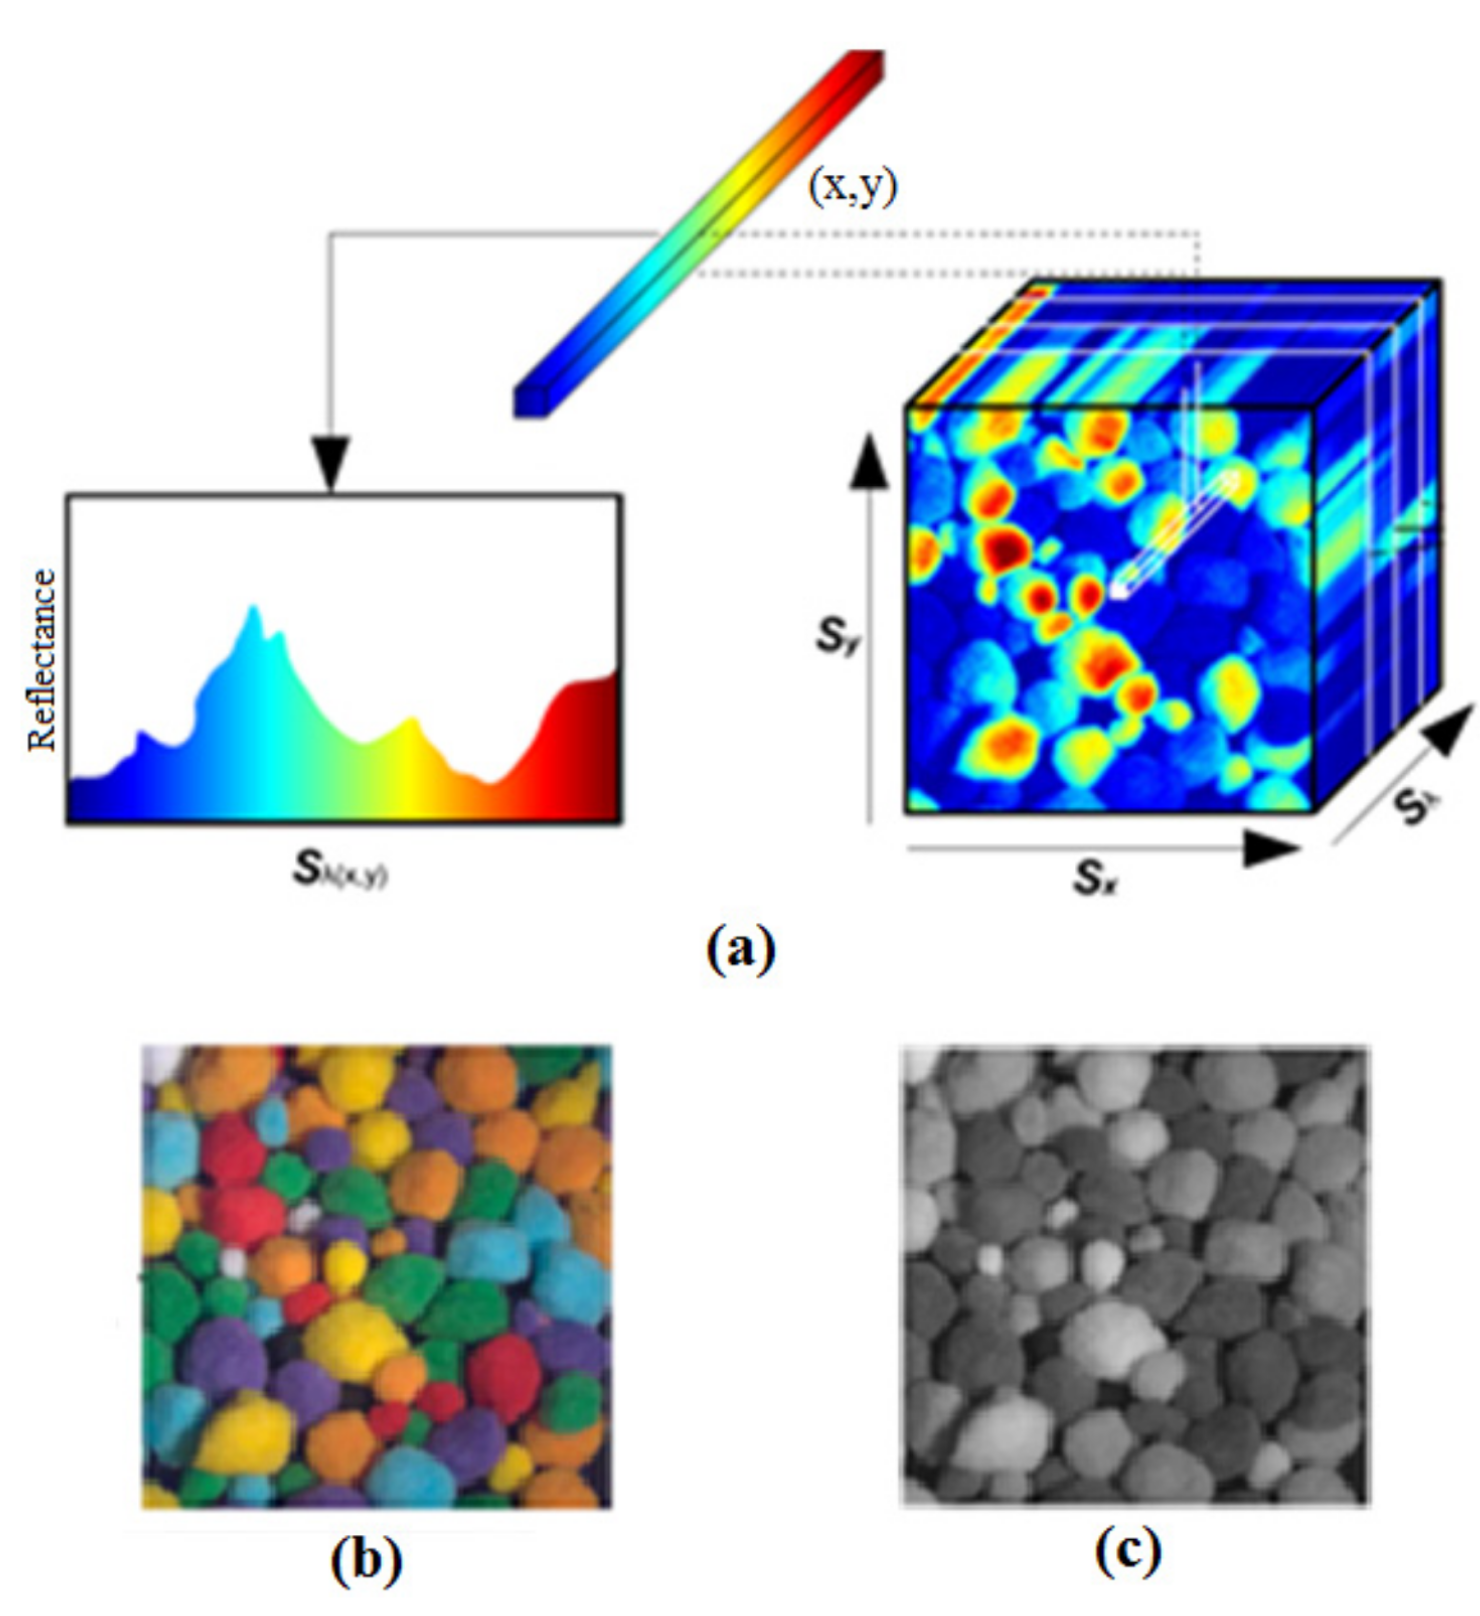
\includegraphics[width=1\linewidth]{HSI_example.png}
            \captionsetup{labelformat=simple, labelsep=colon, font=tiny, labelfont={color=gray,bf}}
            \caption{(a) A hyperspectral image represented as a 3D cube. A point spectrum on the spectral cube is illustrated at the spatial location (x,y). (b) An RGB image and (c) a grayscale image rendered from the hyperspectral cube.\cite{khanModernTrendsHyperspectral2018}}
            \label{fig:khan-modern}
            \end{figure}
        \end{column}

        % Right column
        \begin{column}{0.62\textwidth}
            \begin{itemize}
                \item \small \textbf{Hyperspectral Imaging (HSI)} is a technique that captures image data at multiple wavelengths across the electromagnetic spectrum, providing detailed spectral information for each pixel.
                \item \small \textbf{Unsupervised Clustering} involves grouping pixels in HSI data without prior labels, identifying natural structures and patterns in the data.
                \item \small By applying unsupervised clustering to HSI, we aim to detect distinct materials and features within images, enhancing applications in agriculture, remote sensing, and medical diagnostics.
            \end{itemize}
        \end{column}
    \end{columns}
\end{frame}

\begin{frame}{The Problem to Address}
    \begin{columns}
        % Left column
        \begin{column}{0.38\textwidth}
            \begin{figure}
            \centering
            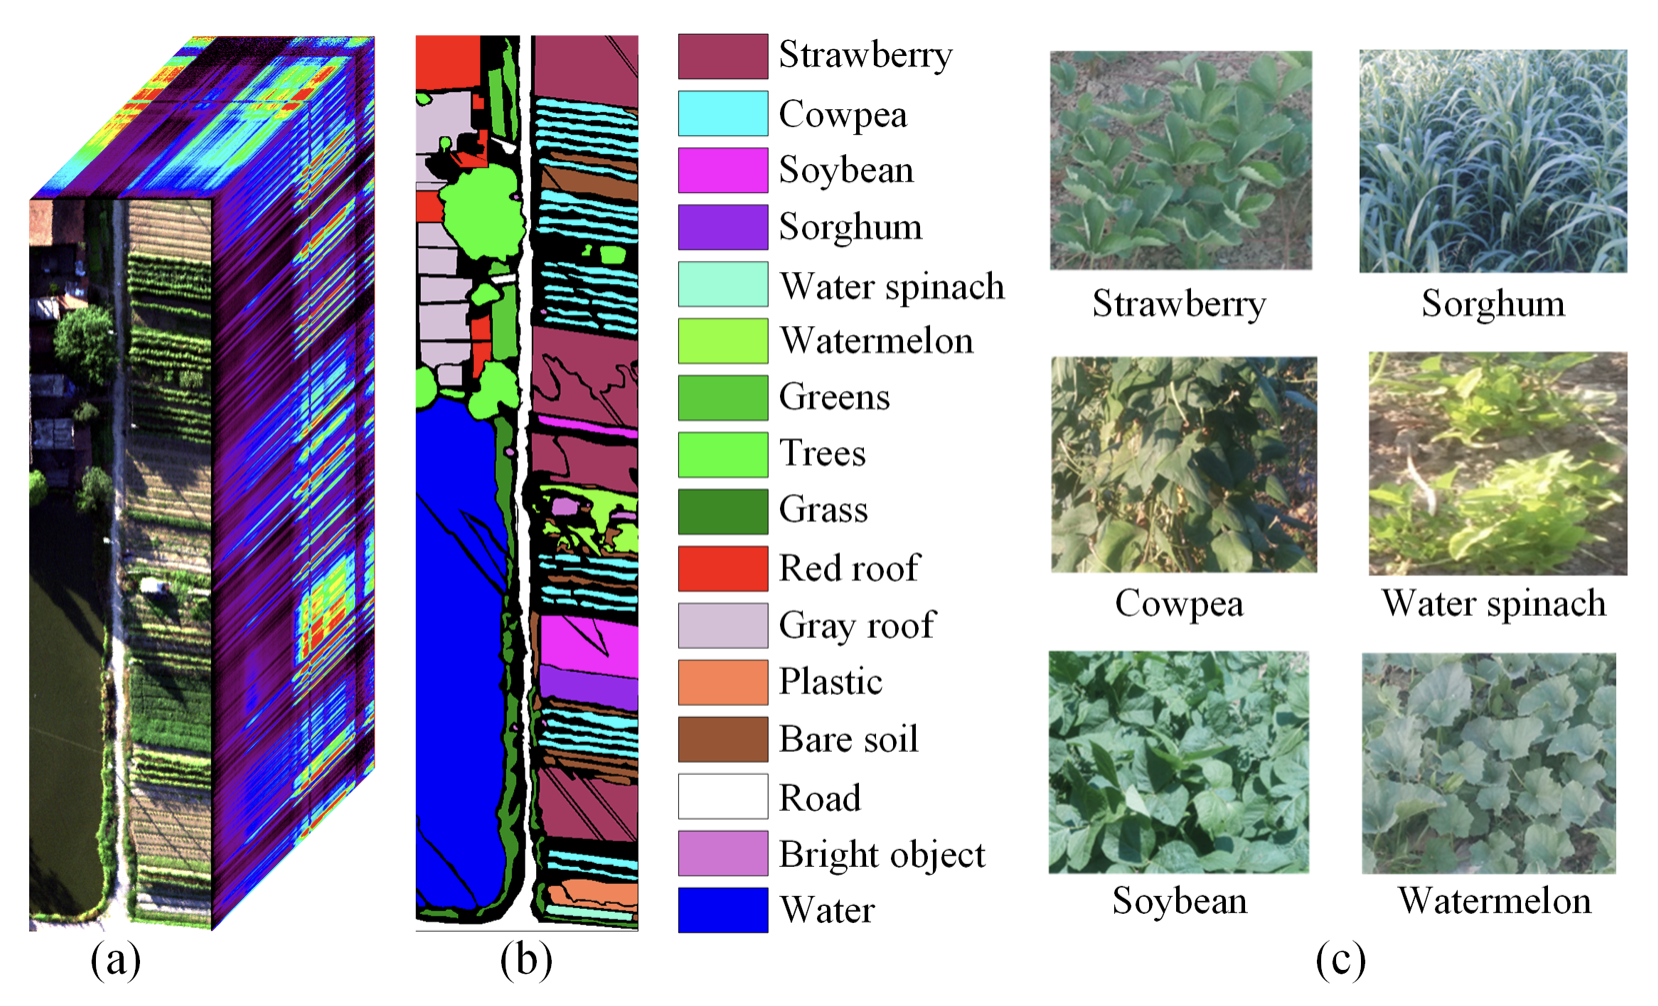
\includegraphics[width=1\linewidth]{WHU-HI_HanChuan274.png}
            \captionsetup{labelformat=simple, labelsep=colon, font=tiny, labelfont={color=gray,bf}}
            \caption{The WHU-Hi-HanChuan dataset was acquired on June 17, 2016, using a UAV-borne hyperspectral imaging sensor. The dataset covers a rural-urban fringe zone and includes seven crop species: strawberry, cowpea, soybean, sorghum, water spinach, watermelon, and greens. The image size is 1217 × 303 pixels, with 274 bands ranging from 400 to 1000 nm. (a) Hyperspectral image cube, (b) ground-truth image, and (c) typical crop photos in the study area. The high dimensionality and complex spectral patterns present challenges for unsupervised clustering and feature extraction.\cite{huWHUHiUAVborneHyperspectral}}
            \label{fig:whu-hi-hanchuan}
            \end{figure}
        \end{column}
        
        % Right column
        \begin{column}{0.62\textwidth}
            \begin{itemize}
                \item \small \textbf{High Dimensionality}: HSI data consists of hundreds of spectral bands, making it computationally challenging to process.
                \item \small \textbf{Complex Patterns}: The spectral information in HSI often includes overlapping and mixed signatures, complicating the clustering process.
                \item \small \textbf{Need for Effective Algorithms}: There is a pressing need for advanced unsupervised clustering algorithms that can efficiently handle the high dimensionality and complexity of HSI data.
            \end{itemize}
        \end{column}
    \end{columns}
\end{frame}

\section{State of the Art (SOTA)}

\subsection{HSI}
\begin{frame}{}
\tiny
\begin{figure}
    \centering
    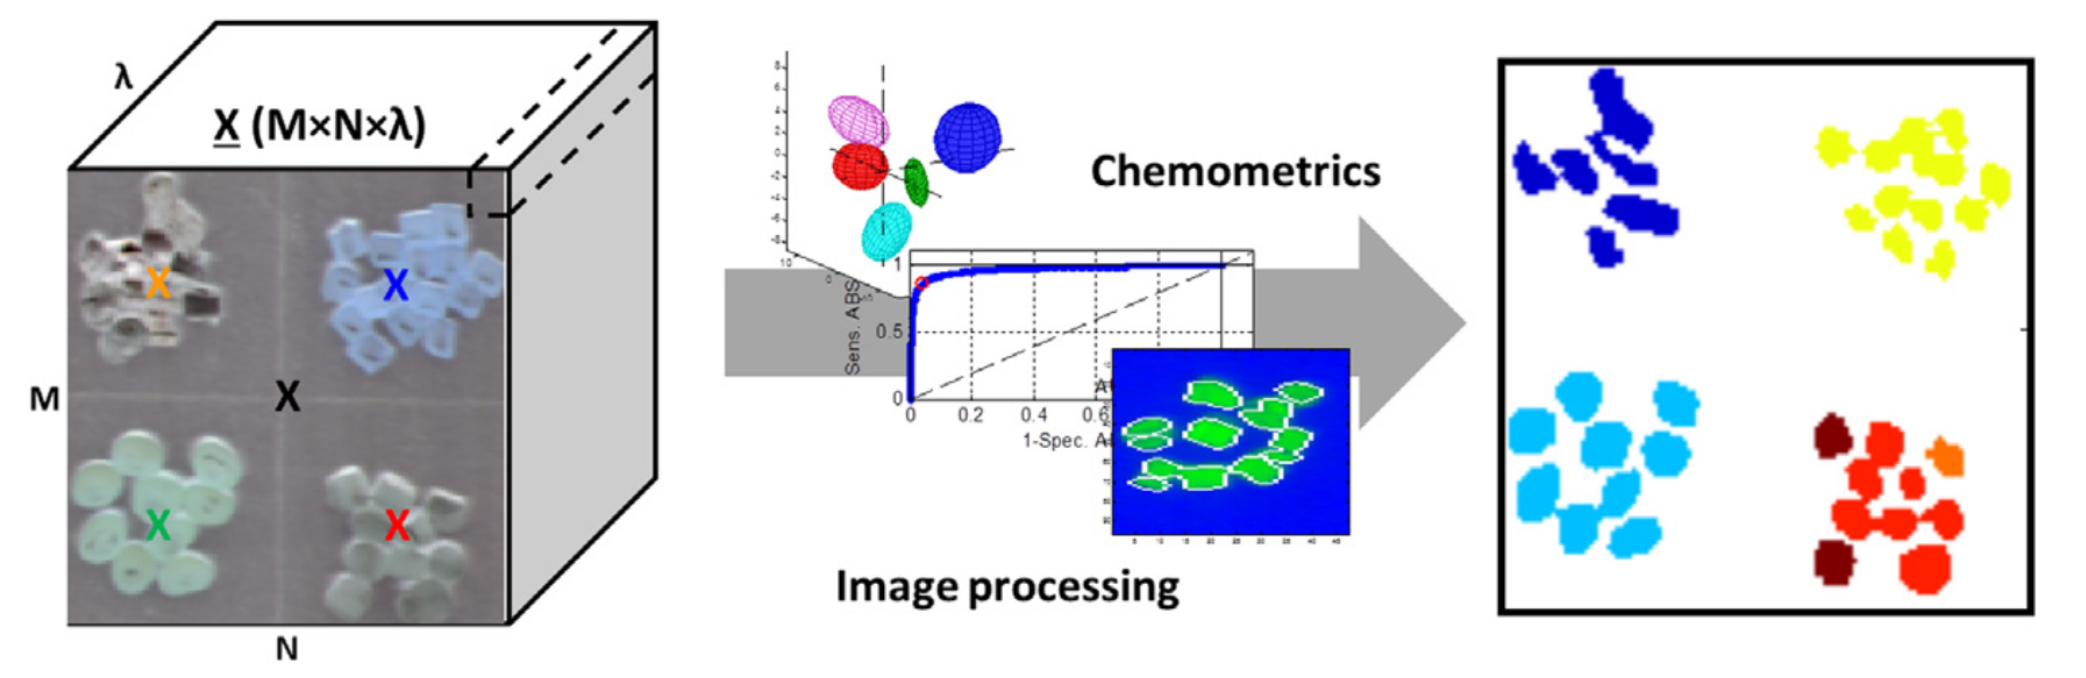
\includegraphics[width=0.62\linewidth]{tutorial_figure.png}
    \captionsetup{labelformat=simple, labelsep=colon, font=tiny, labelfont={color=gray,bf}}
    \caption{\textbf{Graphical Abstract from “Hyperspectral image analysis. A tutorial”} This figure illustrates the hierarchical discrimination of six classes of plastics containing flame retardant using multivariate data analysis and digital image processing methods.\cite{amigoHyperspectralImageAnalysis2015}}
    \label{fig:tutorial_figure}
\end{figure}
\vspace{-0.5cm}
\begin{itemize}
    \item Amigo, J.M., Babamoradi, H., Elcoroaristizabal, S. (2015). Hyperspectral Image Analysis: A Tutorial. \textit{Analytica Chimica Acta}, 896, 34-51. \href{https://www.sciencedirect.com/science/article/pii/S0003267015011691}{\color{blue}{DOI: 10.1016/j.aca.2015.09.030}}
    \cite{amigoHyperspectralImageAnalysis2015}
    
    {\color{gray}Provides guidelines and practical tools for analyzing hyperspectral images, focusing on steps like image acquisition, pre-processing, multivariate exploratory analysis, and classification.}
    \begin{itemize} \tiny
    \item \textbf{PLS-DA Model:} Uses Partial Least Squares Discriminant Analysis (PLS-DA) for classification. The model predicts class membership based on the dummy matrix \( \mathbf{D} \), containing binary entries.
    \[
    \hat{\mathbf{Y}} = \mathbf{X} \mathbf{B}
    \]
    Where \( \hat{\mathbf{Y}} \) is the predicted response, \( \mathbf{X} \) is the data matrix, and \( \mathbf{B} \) is the matrix of regression coefficients.
    \item \textbf{Root Mean Square Error (RMSE):} Measures the optimal number of latent variables (LVs).
    \[
    \text{RMSE} = \sqrt{\frac{1}{n} \sum_{i=1}^{n} (\hat{y}_i - y_i)^2}
    \]
    \item \textbf{Classification Metrics:} Includes sensitivity, specificity, and classification error.
    \[
    \text{Sensitivity} = \frac{\text{TP}}{\text{TP} + \text{FN}}, \quad \text{Specificity} = \frac{\text{TN}}{\text{TN} + \text{FP}}, \quad \text{Class Error} = \frac{\text{FP} + \text{FN}}{\text{Total Samples}}
    \]
\end{itemize}

\end{itemize}
\end{frame}
\begin{frame}{}
\tiny
\begin{itemize}

    \item Prasad, S., Chanussot, J., Fowler, J. E., Bioucas-Dias, J., & Creusere, C. D. (2015). Introduction to the Issue on Advances in Hyperspectral Data Processing and Analysis. \textit{IEEE Journal of Selected Topics in Signal Processing}, 9(6), 961-964. \href{https://doi.org/10.1109/JSTSP.2015.2457631}{\color{blue}{DOI: 10.1109/JSTSP.2015.2457631}}.
    \cite{prasadIntroductionIssueAdvances2015}
    
    {\color{gray}This special issue covers advances in hyperspectral image-processing research, focusing on novel algorithmic approaches, theoretical insights, and performance limits in image-processing techniques.}
    \begin{itemize} \tiny
    \item \textbf{Parallel Processing:} Implements parallel versions of hyperspectral image processing algorithms to handle large datasets efficiently.
    \[
    S(p) = \frac{T(1)}{T(p)}
    \]
    Where \( S(p) \) is the speedup with \( p \) processors, \( T(1) \) is the execution time with one processor, and \( T(p) \) is the execution time with \( p \) processors.
    \item \textbf{Hierarchical Segmentation:} Segments the image at different levels of detail using region-growing and spectral clustering methods. The convergence criterion for region growing is based on minimizing the within-segment variance.
    \[
    E(S) = \sum_{i=1}^{n} \sum_{x_j \in S_i} (\mathbf{x}_j - \boldsymbol{\mu}_i)^T (\mathbf{x}_j - \boldsymbol{\mu}_i)
    \]
    Where \( S \) is the segmentation, \( S_i \) is the \( i \)-th segment, \( \mathbf{x}_j \) is the \( j \)-th pixel, and \( \boldsymbol{\mu}_i \) is the mean vector of segment \( S_i \).
    \item \textbf{Spectral Mixture Analysis:} Decomposes each pixel's spectrum into a linear combination of endmember spectra.
    \[
    \mathbf{r} = \sum_{i=1}^{n} f_i \mathbf{e}_i
    \]
    Where \( \mathbf{r} \) is the reflectance vector, \( f_i \) are the fractional abundances, and \( \mathbf{e}_i \) are the endmember spectra.
\end{itemize}
    
\end{itemize}
\end{frame}
\begin{frame}{}
\tiny
\begin{itemize}

    \item Plaza, A., Benediktsson, J.A., Boardman, J.W., et al. (2009). Recent Advances in Techniques for Hyperspectral Image Processing. \textit{Remote Sensing of Environment}, 113, S110-S122. \href{https://www.sciencedirect.com/science/article/pii/S0034425709000807}{\color{blue}{DOI: 10.1016/j.rse.2009.01.007}}
    \cite{plazaRecentAdvancesTechniques2009}
    
    {\color{gray}Provides an overview of recent techniques in hyperspectral image processing, focusing on high-dimensional data handling and the integration of spatial and spectral information.}
    \begin{itemize} \tiny
    \item \textbf{Hierarchical Segmentation:} Segments the image at different levels of detail using region-growing and spectral clustering methods. The convergence criterion for region growing is based on minimizing the within-segment variance.
    \item \textbf{Parallel Processing:} Implements parallel versions of hyperspectral image processing algorithms to handle large datasets efficiently. The speedup is calculated as: \( S(p) = \frac{T(1)}{T(p)} \), where \( T(1) \) is the execution time with one processor and \( T(p) \) is the execution time with \( p \) processors.
    \item \textbf{Kernel Methods:} Kernel-based methods, such as Support Vector Machines (SVM), are used for classification tasks in hyperspectral imaging. The kernel function \( K(x_i, x_j) \) transforms data into a higher-dimensional space to find a hyperplane that maximizes the margin between classes.
    \[
    K(x_i, x_j) = \phi(x_i) \cdot \phi(x_j)
    \]
    \item \textbf{Markov Random Fields (MRF):} MRFs are used to incorporate spatial context in the classification process by modeling the spatial dependencies between neighboring pixels.
    \[
    P(X = x) = \frac{1}{Z} \exp\left( - \sum_{c \in C} \psi_c(x_c) \right)
    \]
    Where \( Z \) is the partition function, \( \psi_c \) are the potential functions over cliques \( c \).
    \item \textbf{Spectral Mixture Analysis:} This technique decomposes each pixel's spectrum into a linear combination of endmember spectra.
    \[
    \mathbf{r} = \sum_{i=1}^{n} f_i \mathbf{e}_i
    \]
    Where \( \mathbf{r} \) is the reflectance vector, \( f_i \) are the fractional abundances, and \( \mathbf{e}_i \) are the endmember spectra.
\end{itemize}

\end{itemize}
\end{frame}
\begin{frame}{}
\tiny
\begin{itemize}

   \item Khan, M. J., Khan, H. S., Yousaf, A., Khurshid, K., & Abbas, A. (2018). Modern Trends in Hyperspectral Image Analysis: A Review. \textit{IEEE Access}, 6, 14118-14129. \href{https://doi.org/10.1109/ACCESS.2018.2812999}{\color{blue}{DOI: 10.1109/ACCESS.2018.2812999}}.
   \cite{khanModernTrendsHyperspectral2018}
   
    {\color{gray}Reviews modern trends in hyperspectral image analysis, including applications in food quality assessment, medical diagnosis, and forensic science.}
    \begin{itemize} \tiny
    \item \textbf{Data Fusion:} Combines data from multiple sources to improve accuracy and reliability.
    \[
    \mathbf{D}_{fused} = f(\mathbf{D}_1, \mathbf{D}_2, \ldots, \mathbf{D}_n)
    \]
    Where \( \mathbf{D}_{fused} \) is the fused dataset, and \( f \) is the fusion function.
    \item \textbf{Anomaly Detection:} Identifies outliers in hyperspectral images.
    \[
    \text{Anomaly Score} = \frac{(\mathbf{x} - \boldsymbol{\mu})^T \boldsymbol{\Sigma}^{-1} (\mathbf{x} - \boldsymbol{\mu})}{\sqrt{2 \pi |\boldsymbol{\Sigma}|}}
    \]
    Where \( \mathbf{x} \) is the pixel vector, \( \boldsymbol{\mu} \) is the mean vector, and \( \boldsymbol{\Sigma} \) is the covariance matrix.
    \item \textbf{Hyperspectral Unmixing:} Decomposes mixed pixels into their constituent endmember spectra and corresponding abundances.
    \[
    \mathbf{R} = \mathbf{EA} + \mathbf{N}
    \]
    Where \( \mathbf{R} \) is the reflectance matrix, \( \mathbf{E} \) is the endmember matrix, \( \mathbf{A} \) is the abundance matrix, and \( \mathbf{N} \) is the noise matrix.
\end{itemize}

\end{itemize}
\end{frame}
\begin{frame}{}
\tiny
\begin{itemize}

    \item Vidal, M., \& Amigo, J. M. (2012). Pre-processing of Hyperspectral Images: Essential Steps Before Image Analysis. \textit{Chemometrics and Intelligent Laboratory Systems}, 117, 138-148. \href{https://doi.org/10.1016/j.chemolab.2012.05.009}{\color{blue}{DOI: 10.1016/j.chemolab.2012.05.009}}. \cite{vidalPreprocessingHyperspectralImages2012}
    
    {\color{gray}Discusses the necessary pre-processing steps for hyperspectral images, such as background removal and image compression, to enhance data analysis.}
    \begin{itemize} \tiny
    \item \textbf{Image Compression:} Uses methods like PCA (Principal Component Analysis) for data compression.
    \[
    \mathbf{X} \approx \mathbf{T} \mathbf{P}^T
    \]
    Where \( \mathbf{X} \) is the original data matrix, \( \mathbf{T} \) are the scores, and \( \mathbf{P} \) are the loadings.
    \item \textbf{Wavelet Transform:} Applies wavelet transform for noise reduction and data compression.
    \[
    f(t) = \sum_{k=1}^{n} c_k \psi_k(t)
    \]
    Where \( c_k \) are wavelet coefficients and \( \psi_k(t) \) are wavelet functions.
    \item \textbf{Background Removal:} Utilizes thresholding based on PCA scores to distinguish sample from background.
    \[
    \text{Threshold} = \text{mean}(\mathbf{T}) + k \cdot \text{std}(\mathbf{T})
    \]
\end{itemize}
    
\end{itemize}
\end{frame}
\begin{frame}{}
\tiny
\begin{itemize}

    \item Camps-Valls, G., \& Bruzzone, L. (2005). Kernel-Based Methods for Hyperspectral Image Classification. \textit{IEEE Transactions on Geoscience and Remote Sensing}, 43(6), 1351-1362. \href{https://doi.org/10.1109/TGRS.2005.846154}{\color{blue}{DOI: 10.1109/TGRS.2005.846154}}.
    \cite{camps-vallsKernelbasedMethodsHyperspectral2005}
    
    {\color{gray}Presents the framework of kernel-based methods for hyperspectral image classification, comparing different approaches and analyzing their properties in the hyperspectral domain.}
    \begin{itemize} \tiny
    \item \textbf{Support Vector Machines (SVM):} Uses a decision function for classification.
    \[
    f(x) = \sum_{i=1}^{n} \alpha_i y_i K(x_i, x) + b
    \]
    Where \( \alpha_i \) are the Lagrange multipliers, \( y_i \) are the class labels, \( K \) is the kernel function, and \( b \) is the bias term.
    \item \textbf{Kernel Fisher Discriminant (KFD):} Projects data onto a direction that maximizes class separability.
    \[
    J(w) = \frac{w^T S_B w}{w^T S_W w}
    \]
    Where \( S_B \) is the between-class scatter matrix, and \( S_W \) is the within-class scatter matrix.
    \item \textbf{Least Squares SVM (LS-SVM):} Solves a set of linear equations for optimization.
    \[
    \min_w \frac{1}{2} w^T w + \frac{\gamma}{2} \sum_{i=1}^{n} e_i^2 \quad \text{subject to} \quad y_i (w^T \phi(x_i) + b) = 1 - e_i
    \]
    Where \( \gamma \) is the regularization parameter, and \( e_i \) are the error variables.
\end{itemize}
    
\end{itemize}
\end{frame}
\begin{frame}{}
\tiny
\begin{itemize}

    \item Selci, S. (2019). The Future of Hyperspectral Imaging. \textit{Journal of Imaging}, 5(11), 84. \href{https://doi.org/10.3390/jimaging5110084}{\color{blue}{DOI: 10.3390/jimaging5110084}}.
    \cite{selciFutureHyperspectralImaging2019}
    
    {\color{gray}Discusses the current advancements and future trends in hyperspectral imaging (HSI) technology, including applications in medical imaging, agriculture, and cultural heritage, as well as the development of new algorithms and hardware for improved data acquisition and analysis.}
    \begin{itemize} \tiny
    \item \textbf{Spectral Data Fusion:} Combines spectral data from different sources using methods like partial least squares regression (PLSR).
    \[
    \mathbf{Y} = \mathbf{X}\mathbf{B} + \mathbf{E}
    \]
    where \(\mathbf{Y}\) is the dependent variable matrix, \(\mathbf{X}\) is the independent variable matrix, \(\mathbf{B}\) is the regression coefficient matrix, and \(\mathbf{E}\) is the error matrix.
    \item \textbf{Principal Component Analysis (PCA):} Used for dimensionality reduction in hyperspectral data.
    \[
    \mathbf{X} = \mathbf{TP}^T + \mathbf{E}
    \]
    where \(\mathbf{X}\) is the data matrix, \(\mathbf{T}\) are the scores, \(\mathbf{P}\) are the loadings, and \(\mathbf{E}\) is the residual matrix.
    \item \textbf{Classification Techniques:} Methods like k-nearest neighbors (KNN) and support vector machines (SVM) are used for classification tasks.
    \begin{itemize} \tiny
        \item \textbf{KNN:}
        \[
        d(x, y) = \sqrt{\sum_{i=1}^{n} (x_i - y_i)^2}
        \]
        where \(d(x, y)\) is the distance between points \(x\) and \(y\).
        \item \textbf{SVM:}
        \[
        f(x) = \sum_{i=1}^{n} \alpha_i y_i K(x_i, x) + b
        \]
        where \(\alpha_i\) are the Lagrange multipliers, \(y_i\) are the class labels, \(K\) is the kernel function, and \(b\) is the bias term.
    \end{itemize}
    \item \textbf{Image Registration:} Aligns hyperspectral images taken at different times or from different sensors.
    \[
    \text{MI}(A, B) = \sum_{a \in A} \sum_{b \in B} p(a, b) \log \frac{p(a, b)}{p(a)p(b)}
    \]
    where \(\text{MI}(A, B)\) is the mutual information between images \(A\) and \(B\).
\end{itemize}

\end{itemize}
\end{frame}
\begin{frame}
\tiny
\begin{figure}
    \centering
            \centering
            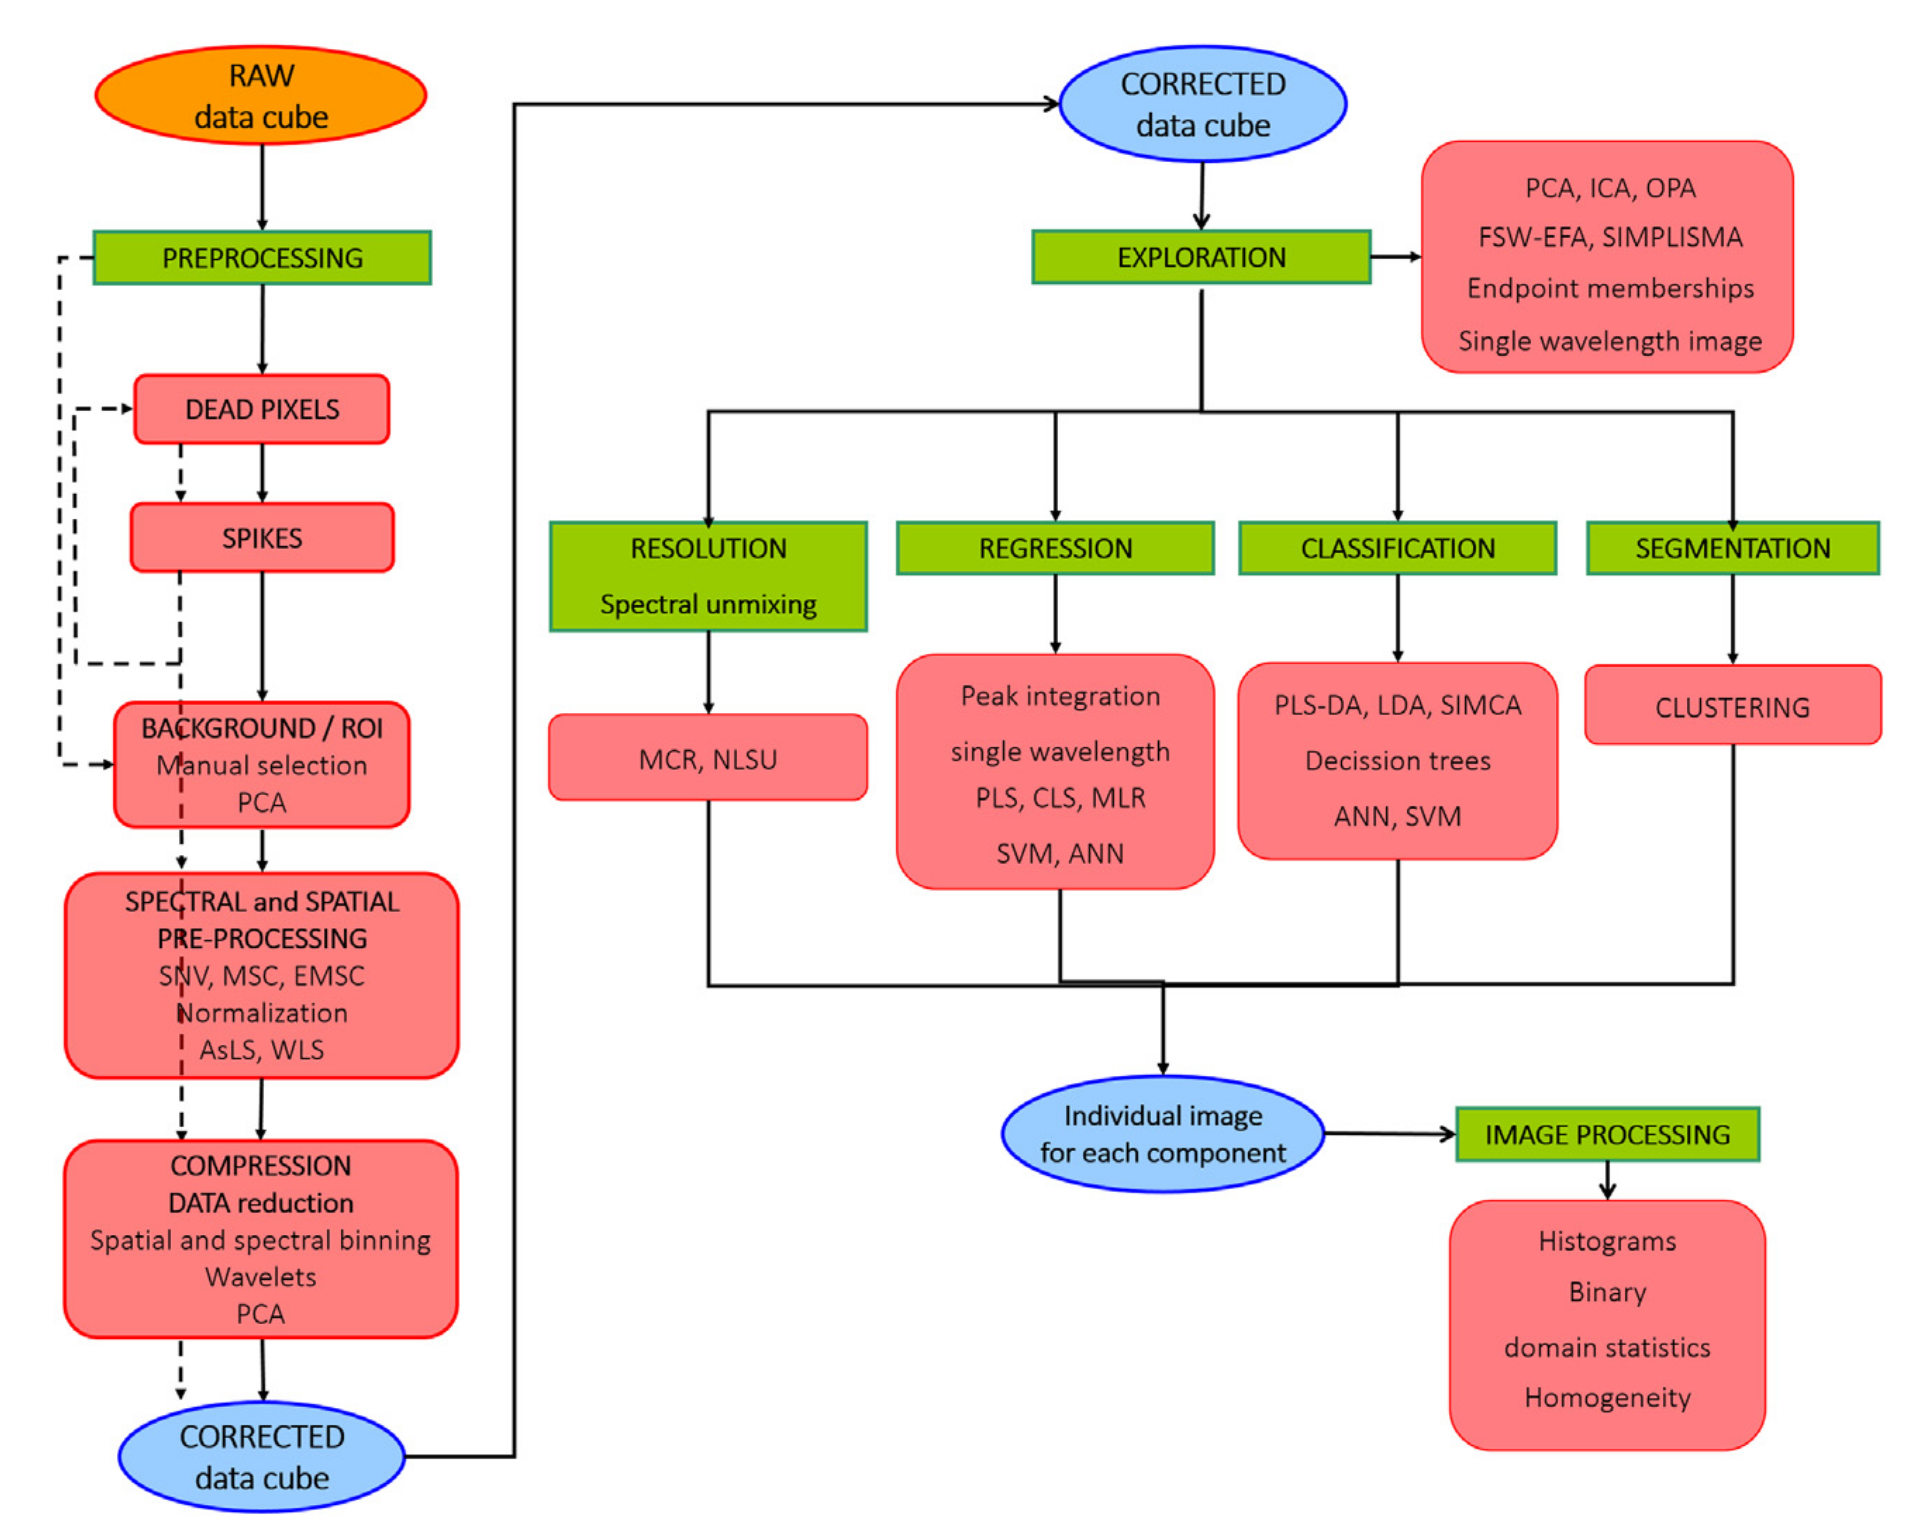
\includegraphics[width=0.62\linewidth]{amigo_chart.png}
            \captionsetup{labelformat=simple, labelsep=colon, font=tiny, labelfont={color=gray,bf}}
            \caption{\textbf{Comprehensive Flowchart of Hyperspectral and Multispectral Image Analysis} This flowchart outlines the complete process of hyperspectral and multispectral image analysis. It begins with preprocessing the raw data cube, addressing issues like dead pixels and spikes, and includes steps such as spectral and spatial preprocessing, data compression, and correction. The corrected data cube is then explored using techniques like PCA, ICA, and SIMPLISMA. The analysis continues with resolution (spectral unmixing), regression (peak integration, PLS, SVM), classification (PLS-DA, LDA, ANN), and segmentation (clustering). The final stage involves image processing for histogram analysis, binary domain statistics, and homogeneity. (Adapted from Amigo et al., 2015)\cite{amigoHyperspectralMultispectralImaging2019}}
    \label{fig:amigo_chart}
\end{figure}

\end{frame}
\begin{frame}
\tiny
\begin{itemize}

\item Amigo, J.M. (2019). Hyperspectral and Multispectral Imaging: Setting the Scene. \textit{Hyperspectral Imaging}. Elsevier. \href{https://doi.org/10.1016/B978-0-444-63977-6.00001-8}{\color{blue}{DOI: 10.1016/B978-0-444-63977-6.00001-8}}
\cite{amigoHyperspectralMultispectralImaging2019}

{\color{gray}Discusses the basic concepts of hyperspectral and multispectral imaging, including spatial resolution, types of images, data mining, and chemometrics.}
\begin{itemize} \tiny
    \item \textbf{Spatial Resolution:}
    \[
    \text{Resolution} = \frac{\text{Image Size}}{\text{Pixel Size}}
    \]
    \item \textbf{Single Channel Images:}
    \[
    I(x, y)
    \]
    \item \textbf{Color-Space Images:}
    \[
    \text{RGB} = (R, G, B)
    \]
    \item \textbf{Multiband Images:}
    \[
    \{I_{\lambda_1}, I_{\lambda_2}, \ldots, I_{\lambda_n}\}
    \]
    \item \textbf{Hyperspectral Images:}
    \[
    \{I(\lambda_1), I(\lambda_2), \ldots, I(\lambda_n)\}
    \]
    \item \textbf{Chemometrics:}
    \[
    \text{Hypercube} = (X \times Y \times \lambda)
    \]
    \item \textbf{Preprocessing:}
    \[
    I_{\text{normalized}} = \frac{I_{\text{raw}} - I_{\text{dark}}}{I_{\text{white}} - I_{\text{dark}}}
    \]
    \item \textbf{Pattern Recognition/Exploration:}
    \[
    \mathbf{X} = \mathbf{T} \mathbf{P}^T + \mathbf{E}
    \]
    \item \textbf{Segmentation:}
    \[
    \min \sum_{i=1}^{k} \sum_{x_j \in C_i} \|x_j - \mu_i\|^2
    \]
    \item \textbf{Curve Resolution Methods/Spectral Unmixing:}
    \[
    \mathbf{D} = \mathbf{C} \mathbf{S} + \mathbf{E}
    \]
    \item \textbf{Regression and Classification:}
    \[
    \mathbf{Y} = \mathbf{X} \mathbf{B}
    \]
\end{itemize}

\end{itemize}
\end{frame}
\begin{frame}
\tiny
\begin{itemize}

 \item Manolakis, D., \& Shaw, G. (2002). Detection Algorithms for Hyperspectral Imaging Applications. \textit{IEEE Signal Processing Magazine}, 19(1), 29-43. \href{https://doi.org/10.1109/79.911197}{\color{blue}{DOI: 10.1109/79.911197}}. \cite{manolakisDetectionAlgorithmsHyperspectral2002}

    {\color{gray}Discusses the development and evaluation of hyperspectral target detection algorithms using statistical hypothesis testing, focusing on the likelihood ratio test (LRT), quadratic detectors, adaptive matched filters (AMF), and spectral angle mapper (SAM), and addressing the challenges of spectral variability and mixed pixels.}
    \begin{itemize} \tiny
    \item \textbf{Likelihood Ratio Test (LRT):}
    \[
    \Lambda(x) = \frac{p(x|\text{signal present})}{p(x|\text{signal absent})}
    \]
    where \(\Lambda(x)\) is the likelihood ratio, and \(p(x)\) are the conditional probability density functions.

    \item \textbf{Quadratic Detector:}
    \[
    y = x^T \Sigma_b^{-1} \mu_b - x^T \Sigma_t^{-1} \mu_t - \frac{1}{2} \left( \mu_b^T \Sigma_b^{-1} \mu_b - \mu_t^T \Sigma_t^{-1} \mu_t \right)
    \]
    where \(x\) is the observed spectrum, \(\mu_b\) and \(\mu_t\) are the mean vectors, and \(\Sigma_b\) and \(\Sigma_t\) are the covariance matrices of the background and target classes.

    \item \textbf{Adaptive Matched Filter (AMF):}
    \[
    y = \frac{s^T \Sigma_b^{-1} x}{s^T \Sigma_b^{-1} s}
    \]
    where \(s\) is the target signature vector and \(\Sigma_b\) is the background covariance matrix.

    \item \textbf{Spectral Angle Mapper (SAM):}
    \[
    \theta = \cos^{-1} \left( \frac{x^T s}{\|x\| \|s\|} \right)
    \]
    where \(\theta\) is the spectral angle between the test pixel \(x\) and the target signature \(s\).
    \end{itemize}

\end{itemize}
\end{frame}
\begin{frame}{}
\tiny
\begin{itemize}

    \item Landgrebe, D. (2002). Hyperspectral Image Data Analysis. \textit{IEEE Signal Processing Magazine}, 18(1), 17-28. \href{https://ieeexplore.ieee.org/document/1352410}{\color{blue}{DOI: 10.1109/79.939829}} \cite{landgrebeHyperspectralImageData2002}
    
    {\color{gray}Discusses the evolution and techniques of hyperspectral image data analysis, highlighting the multispectral approach and its applications in remote sensing.}
    \begin{itemize} \tiny
    \item \textbf{Class Density Functions:} Uses discriminant functions for classification. For two classes with means \( \mu_f \) and \( \mu_g \) and covariance matrices \( \Sigma_f \) and \( \Sigma_g \), the quadratic classifier is: \[ g_i(x) = -\frac{1}{2} (x - \mu_i)^T \Sigma_i^{-1} (x - \mu_i) - \frac{1}{2} \log |\Sigma_i| \].
    \item \textbf{Linear Discriminant Analysis (LDA):} Maximizes the ratio of between-class variance to within-class variance: \[ J(w) = \frac{w^T S_b w}{w^T S_w w} \], where \( S_b \) and \( S_w \) are the between-class and within-class scatter matrices.
\end{itemize}

\end{itemize}
\end{frame}
\begin{frame}{}
\tiny
\begin{itemize}

    \item Barnes, M., Pan, Z., Zhang, S. (2015). Systems and Methods for Hyperspectral Imaging. \textit{US Patent 9,117,133}. \href{https://patents.google.com/patent/US9117133B2/en}{\color{blue}{DOI: 10.1109/TGRS.2015.2421060}}
    
    {\color{gray}Describes various systems and methods for hyperspectral imaging, emphasizing the technological advancements and applications in different fields.}
    \begin{itemize} \tiny
    \item \textbf{Neural Networks:} Uses neural networks for classification.
    \[
    J = E + \lambda \|W\|^2
    \]
    Where \( J \) is the new criterion, \( E \) is the training error, \( \lambda \) is the regularization parameter, and \( \|W\| \) is the weight norm.
    \item \textbf{Pruning Algorithms:} Uses Optimal Brain Damage (OBD) and Optimal Brain Surgeon (OBS) for weight elimination.
    \[
    \Delta E \approx \frac{1}{2} \Delta W^T H \Delta W
    \]
    Where \( H \) is the Hessian matrix.
    \item \textbf{Similarity Metrics:} Calculates similarity metrics for spectral signatures.
    \[
    \text{Similarity Metric} = \frac{\sum (x_i - \mu_x)(y_i - \mu_y)}{\sqrt{\sum (x_i - \mu_x)^2 \sum (y_i - \mu_y)^2}}
    \]
\end{itemize}

\end{itemize}
\end{frame}
\begin{frame}{PDF unfound:}
\tiny
\begin{itemize}
    \item Kwon, H., Nasrabadi, N.M., Bandos, T.V., et al. (2013). Algorithms for Multispectral and Hyperspectral Image Analysis. \textit{Journal of Electrical and Computer Engineering}, 2013, Article ID 917203. \href{https://www.hindawi.com/journals/jece/2013/917203/}{\color{blue}{DOI: 10.1155/2013/917203}}
    
    {\color{gray}Focuses on advances in algorithms and technologies for multispectral and hyperspectral imagery, addressing critical issues such as anomaly detection and target classification.}
    
    \item Grahn, H., Geladi, P. (2007). Techniques and Applications of Hyperspectral Image Analysis. \textit{Techniques and Applications of Hyperspectral Image Analysis}, John Wiley \& Sons. \href{https://books.google.com/books?id=2ifVDwAAQBAJ}{\color{blue}{DOI: 10.1002/9780470010861}} 

    {\color{gray}Provides a comprehensive overview of various techniques and applications in hyperspectral image analysis, covering principles of multivariate image analysis, clustering, classification, and calibration standards.}

    \item

    \item Kerekes, J.P., Baum, J.E. (2003). Hyperspectral Imaging System Modeling. \textit{Lincoln Laboratory Journal}, 14(1), 3-32. \href{https://apps.dtic.mil/sti/citations/ADA415477}{\color{blue}{DOI: 10.1109/TGRS.2003.814658}}
    
    {\color{gray}Discusses the modeling of hyperspectral imaging systems, including sensor design, calibration, and performance evaluation.}

    \item Manolakis, D., Marden, D., Kerekes, J.P. (2001). Statistics of Hyperspectral Imaging Data. \textit{SPIE Optical Engineering}, 40(8), 2082-2094. \href{https://www.spiedigitallibrary.org/journals/optical-engineering/volume-40/issue-8/2082/Statistics-of-hyperspectral-imaging-data/10.1117/1.1394690.full}{\color{blue}{DOI: 10.1117/1.1394690}}
    
    {\color{gray}Analyzes the statistical properties of hyperspectral imaging data, providing insights into data characterization and noise reduction techniques.}
    
    \item ElMasry, G., Sun, D.W. (2010). Principles of Hyperspectral Imaging Technology. \textit{Hyperspectral Imaging for Food Quality Analysis and Control}, 3-43. \href{https://www.elsevier.com/books/hyperspectral-imaging-for-food-quality-analysis-and-control/sun/978-0-12-374753-2}{\color{blue}{DOI: 10.1016/B978-0-12-374753-2.00001-8}}
    
    {\color{gray}Discusses the principles of hyperspectral imaging technology, focusing on its application in food quality analysis.}
\end{itemize}
\end{frame}














\subsection{Unsupervised Clustering in HSI}
\begin{frame}{}
\tiny
\begin{figure}
    \centering
            \centering
            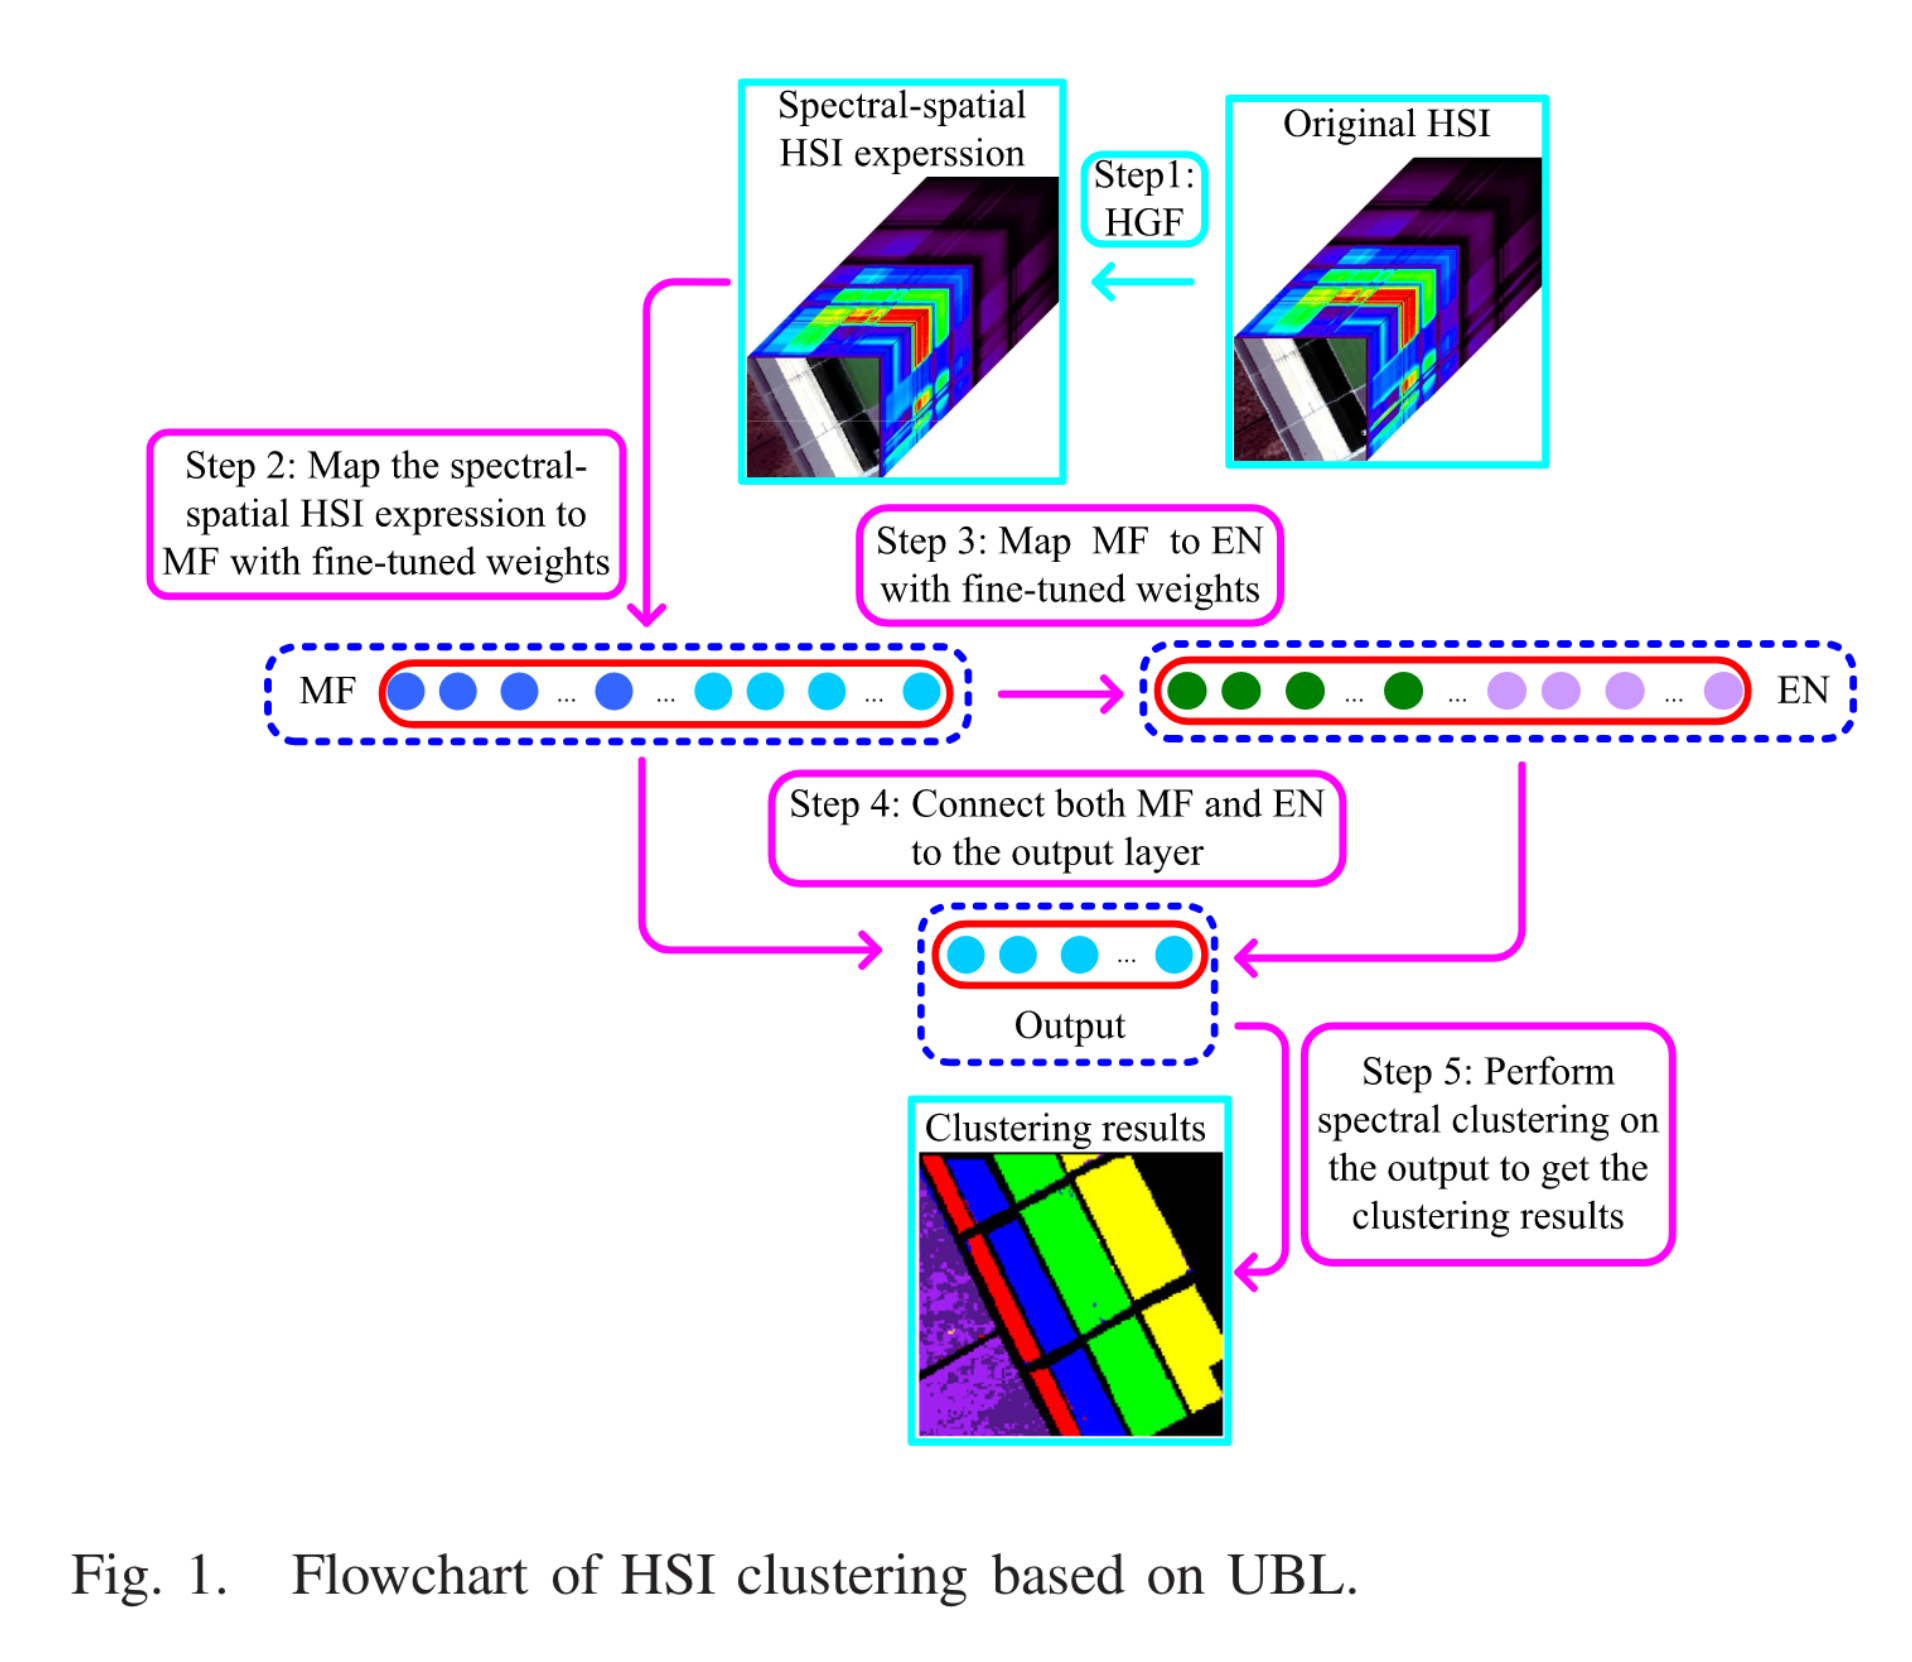
\includegraphics[width=0.62\linewidth]{kong_chat.png}
            \captionsetup{labelformat=simple, labelsep=colon, font=tiny, labelfont={color=gray,bf}}
            \caption{\textbf{Flowchart of HSI Clustering Based on Unsupervised Broad Learning (UBL)} This flowchart illustrates the process of hyperspectral image (HSI) clustering using UBL. Step 1 involves extracting the spectral-spatial HSI expression from the original HSI using hierarchical Gaussian filtering (HGF). In Step 2, the spectral-spatial HSI expression is mapped to the middle feature (MF) layer with fine-tuned weights. Step 3 maps the MF layer to the end feature (EN) layer with fine-tuned weights. Step 4 connects both MF and EN layers to the output layer. Finally, Step 5 performs spectral clustering on the output to obtain the clustering results.\cite{kongHyperspectralImageClustering2019}}
    \label{fig:kong_chart}
\end{figure}
\end{frame}
\begin{frame}
\tiny
\begin{itemize}
\item Kong, Y., Cheng, Y., Chen, C. L. P., \& Wang, X. (2019). Hyperspectral Image Clustering Based on Unsupervised Broad Learning. \textit{IEEE Geoscience and Remote Sensing Letters}, 16(11), 1741-1745. \href{https://doi.org/10.1109/LGRS.2019.2907598}{\color{blue}{DOI: 10.1109/LGRS.2019.2907598}} \cite{kongHyperspectralImageClustering2019}

{\color{gray}Introduces a novel unsupervised broad learning (UBL) method for hyperspectral image clustering, leveraging graph-regularized sparse autoencoders to preserve intrinsic manifold structure.}
\begin{itemize} \tiny
    \item \textbf{Graph-regularized Sparse Autoencoder:}
    \[
    \min_{W, E} \|XW - E\|^2 + \lambda \|W\|_1 + \alpha \text{tr}(E^T L E)
    \]
    where \(X\) is the input data, \(W\) are the weights, \(E\) are the mapped features, \(\lambda\) is the regularization parameter, and \(L\) is the Laplacian matrix.

    \item \textbf{Spectral Clustering:}
    \[
    \min_{W} \|[E|F]W - Y\|^2 + \delta \|W\|^2
    \]
    where \(E\) and \(F\) are the features, \(W\) are the output-layer weights, \(Y\) is the output, and \(\delta\) is the regularization parameter.
\end{itemize}

\end{itemize}
\end{frame}
\begin{frame}{}
\tiny
\begin{itemize}

\item Murphy, J. M., \& Maggioni, M. (2019). Spectral–Spatial Diffusion Geometry for Hyperspectral Image Clustering. \textit{IEEE Geoscience and Remote Sensing Letters}, 17(7), 1243-1247. \href{https://doi.org/10.1109/LGRS.2019.2943001}{\color{blue}{DOI: 10.1109/LGRS.2019.2943001}}. \cite{murphyUnsupervisedClusteringActive2018}

{\color{gray}Proposes an unsupervised learning algorithm for clustering hyperspectral image data using spatially regularized random walks, improving clustering performance by integrating spatial regularity into diffusion processes.}
\begin{itemize} \tiny
    \item \textbf{Diffusion Distance:}
    \[
    d_t(x_i, x_j) = \sqrt{\sum_{k=1}^{n} \left( P_t(i,k) - P_t(j,k) \right)^2 / \pi(k)}
    \]
    where \( d_t(x_i, x_j) \) is the diffusion distance between points \( x_i \) and \( x_j \) at time \( t \), \( P_t \) is the transition matrix, and \( \pi(k) \) is the stationary distribution.

    \item \textbf{Diffusion Maps:}
    \[
    \Phi_t(x) = \left( \lambda_1^t \psi_1(x), \lambda_2^t \psi_2(x), \ldots, \lambda_m^t \psi_m(x) \right)
    \]
    where \( \Phi_t(x) \) is the diffusion map, \( \lambda_i \) are the eigenvalues, and \( \psi_i(x) \) are the corresponding eigenvectors.

    \item \textbf{Kernel Density Estimation (KDE):}
    \[
    f(x) = \frac{1}{n h^d} \sum_{i=1}^{n} K \left( \frac{x - x_i}{h} \right)
    \]
    where \( f(x) \) is the density estimate at point \( x \), \( K \) is the kernel function, \( h \) is the bandwidth, and \( n \) is the number of data points.

    \item \textbf{Mode Detection:}
    \[
    D_t(x) = f(x) \delta_t(x)
    \]
    where \( D_t(x) \) is the mode score, \( f(x) \) is the KDE, and \( \delta_t(x) \) is the distance to the nearest neighbor of higher density.
\end{itemize}
 
\end{itemize}
\end{frame}
\begin{frame}{}
\tiny
\begin{itemize}

\item Zhu, W., Chayes, V., Tiard, A., Sanchez, S., Dahlberg, D., Bertozzi, A. L., Osher, S., Zosso, D., \& Kuang, D. (2017). Unsupervised Classification in Hyperspectral Imagery With Nonlocal Total Variation and Primal-Dual Hybrid Gradient Algorithm. \textit{IEEE Transactions on Geoscience and Remote Sensing}, 55(5), 2786-2797. \href{https://doi.org/10.1109/TGRS.2017.2654486}{\color{blue}{DOI: 10.1109/TGRS.2017.2654486}}. \cite{zhuUnsupervisedClassificationHyperspectral2017}

{\color{gray}Proposes a graph-based nonlocal total variation method for unsupervised classification of hyperspectral images, solved by the primal-dual hybrid gradient algorithm, and demonstrates its superior performance over standard unsupervised clustering methods.}
\begin{itemize} \tiny
    \item \textbf{Total Variation (TV) Model:}
    \[
    E(u) = \| \nabla u \|_{L1} + \lambda S(u)
    \]
    where \( E(u) \) is the energy functional, \( \nabla u \) is the gradient, \( S(u) \) is the data fidelity term, and \( \lambda \) is a regularization parameter.

    \item \textbf{Nonlocal Total Variation (NLTV) Operator:}
    \[
    \nabla_w u(x)(y) = \sqrt{w(x, y)}(u(y) - u(x))
    \]
    where \( w(x, y) \) is the nonlocal weight based on similarity between pixels \( x \) and \( y \).

    \item \textbf{Primal-Dual Hybrid Gradient (PDHG) Algorithm:}
    \[
    \begin{aligned}
    y^{n+1} &= \text{prox}_{\sigma F^*}(y^n + \sigma K \bar{x}^n) \\
    x^{n+1} &= \text{prox}_{\tau G}(x^n - \tau K^* y^{n+1}) \\
    \bar{x}^{n+1} &= x^{n+1} + \theta (x^{n+1} - x^n)
    \end{aligned}
    \]
    where \( K \) is the linear operator, \( F^* \) is the convex conjugate of \( F \), \( \tau \) and \( \sigma \) are step sizes, and \( \theta \) is a parameter.

    \item \textbf{Stable Simplex Clustering:}
    \[
    g(\delta) = -\log \left( \prod_{l=1}^{k} F_l(\delta) \right) + \eta \exp(G(\delta))
    \]
    where \( F_l(\delta) \) is the percentage of data points in cluster \( l \), and \( G(\delta) \) is the percentage of data points on the edges near the division.
\end{itemize}

\end{itemize}
\end{frame}
\begin{frame}{}
\tiny
\begin{itemize}

\item Zhang, S., \& Murphy, J. M. (2021). Hyperspectral Image Clustering with Spatially-Regularized Ultrametrics. \textit{Remote Sensing}, 13(5), 955. \href{https://doi.org/10.3390/rs13050955}{\color{blue}{DOI: 10.3390/rs13050955}} \cite{zhangHyperspectralImageClustering2021}

{\color{gray}Proposes a method for unsupervised clustering of hyperspectral images based on spatially regularized spectral clustering with ultrametric path distances, combining data density and spectral-spatial geometry.}
\begin{itemize} \tiny
    \item \textbf{Ultrametric Path Distances:}
    \[
    d_U(x, y) = \max_{p \in \mathcal{P}(x,y)} \min_{e \in p} w(e)
    \]
    where \(d_U\) is the ultrametric distance, \(\mathcal{P}(x,y)\) is the set of paths between \(x\) and \(y\), and \(w(e)\) is the weight of edge \(e\).
    \item \textbf{Spectral Clustering:}
    \[
    \min_{Z} \text{tr}(Z^T L Z)
    \]
    where \(Z\) is the clustering assignment matrix and \(L\) is the graph Laplacian.
\end{itemize}

\end{itemize}
\end{frame}
\begin{frame}{}
\tiny
\vspace{-0.18cm}
\begin{figure}
    \centering
    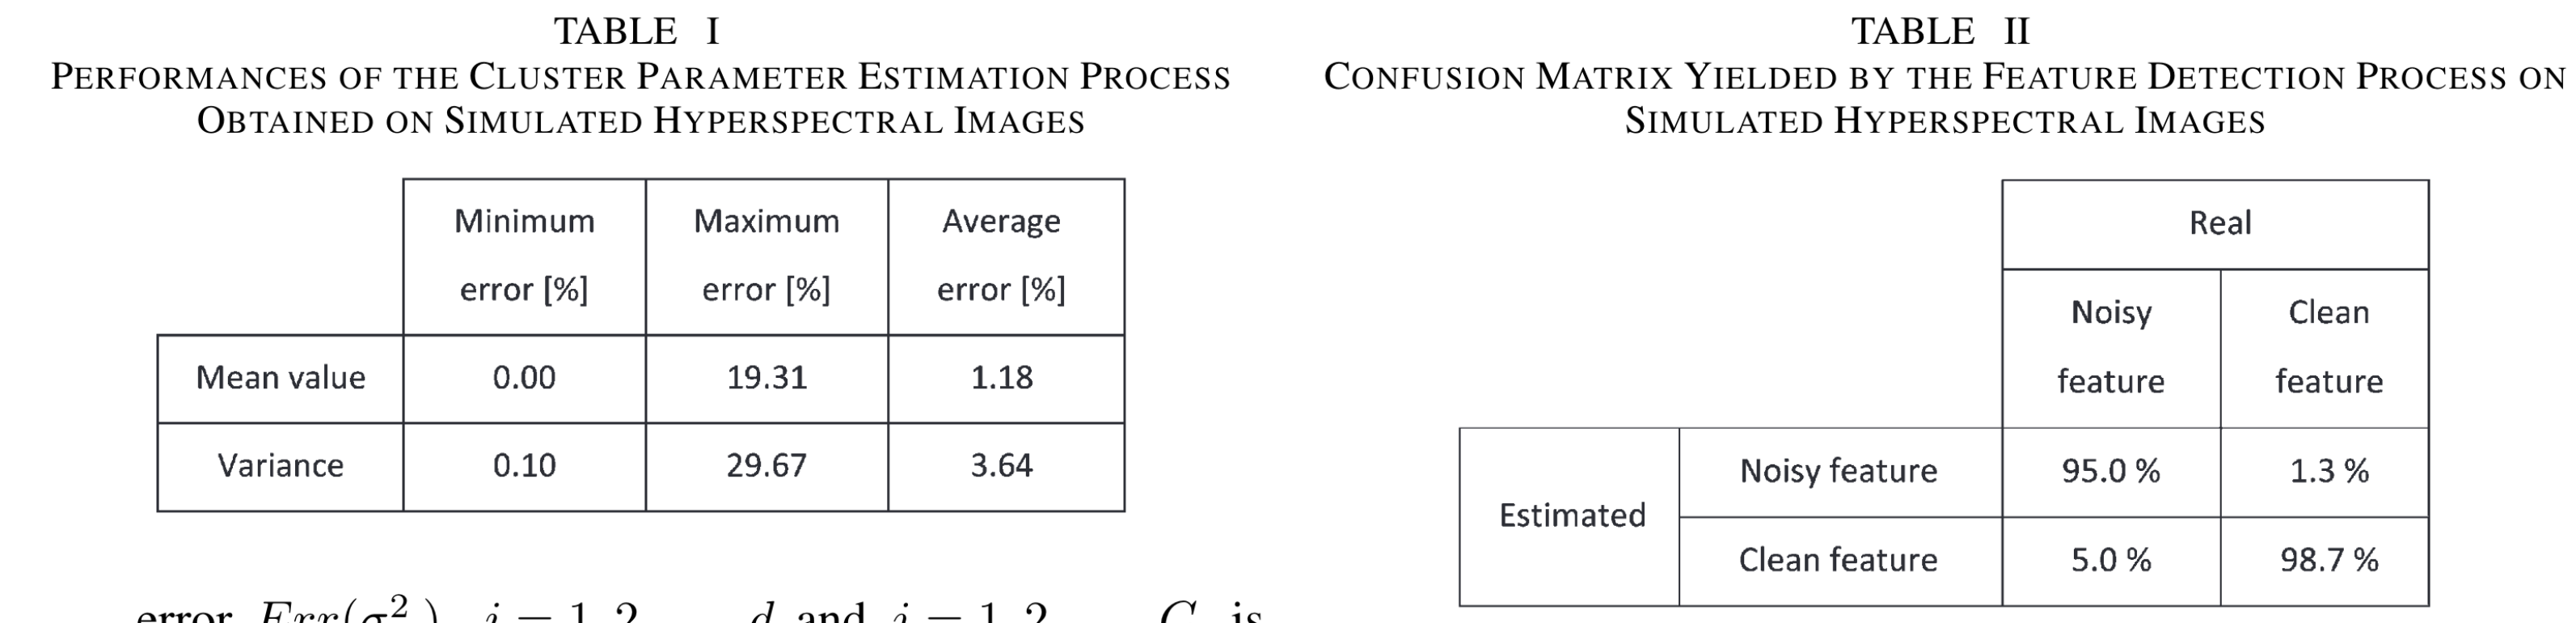
\includegraphics[width=1\linewidth]{paoli_tables.png}
    \captionsetup{labelformat=simple, labelsep=colon, font=tiny, labelfont={color=gray,bf}}
    \caption{\textbf{Performance Metrics and Confusion Matrix for Clustering Hyperspectral Images Using MOPSO} (Paoli et al.)\cite{paoliClusteringHyperspectralImages2009}}
    \label{fig:paoli_tables}
\end{figure}
\vspace{-0.3cm}
\begin{itemize}

    \item Paoli, A., Melgani, F., \& Pasolli, E. (2009). Clustering of Hyperspectral Images Based on Multiobjective Particle Swarm Optimization. \textit{IEEE Transactions on Geoscience and Remote Sensing}, 47(12), 4175-4188. \href{https://doi.org/10.1109/TGRS.2009.2023666}{\color{blue}{DOI: 10.1109/TGRS.2009.2023666}}. \cite{paoliClusteringHyperspectralImages2009}
    
    {\color{gray}Proposes a novel methodology for clustering hyperspectral images using multiobjective particle swarm optimization, addressing class parameter estimation, feature selection, and class number estimation.}
    \begin{itemize} \tiny
    \item \textbf{Multiobjective Particle Swarm Optimization (MOPSO):}
    \(
    \min F(x) = [f_1(x), f_2(x), \ldots, f_m(x)]
    \)
    
    where \( F(x) \) is the objective function vector.
    \item \textbf{Log-Likelihood Function:}
    \(
    L(x|p,Pc) = \sum_{i=1}^{n} \ln \sum_{j=1}^{C} P(\omega_j) \frac{1}{(2\pi)^{d/2} |\Sigma_j|^{1/2}} \exp \left( -\frac{1}{2} (x_i - \mu_j)^T \Sigma_j^{-1} (x_i - \mu_j) \right)
    \)
    
    where \( L \) is the log-likelihood, \( x \) are the data points, \( P(\omega_j) \) are the prior probabilities, \( \Sigma_j \) are the covariance matrices, and \( \mu_j \) are the mean vectors.

    \item \textbf{Bhattacharyya Distance:}
    \(
    B_{ij} = \frac{1}{8} (\mu_i - \mu_j)^T \left( \frac{\Sigma_i + \Sigma_j}{2} \right)^{-1} (\mu_i - \mu_j) + \frac{1}{2} \ln \left( \frac{|\Sigma_i + \Sigma_j|}{2 \sqrt{|\Sigma_i||\Sigma_j|}} \right)
    \)
    
    where \( B_{ij} \) is the Bhattacharyya distance between classes \( i \) and \( j \).

    \item \textbf{Minimum Description Length (MDL):}
    \(
    \text{MDL}(C) = -L(C) + \gamma \cdot K(C) \cdot \log(n)
    \)
    
    where \( L(C) \) is the log-likelihood, \( K(C) \) is the number of estimated parameters, \( n \) is the number of observations, and \( \gamma \) is a constant.
    \end{itemize}
    
\end{itemize}
\end{frame}
\begin{frame}{}
\tiny
\begin{itemize}

    \item Alajlan, N., Bazi, Y., Melgani, F., \& Yager, R. R. (2012). Fusion of Supervised and Unsupervised Learning for Improved Classification of Hyperspectral Images. \textit{Information Sciences}, 217, 39-55. \href{https://doi.org/10.1016/j.ins.2012.06.031}{\color{blue}{DOI: 10.1016/j.ins.2012.06.031}}. \cite{alajlanFusionSupervisedUnsupervised2012}
    
    {\color{gray}Proposes a novel framework combining SVM and FCM clustering to improve hyperspectral image classification by leveraging supervised and unsupervised learning, using Markov Fisher Selector for band selection and various fusion methods for final classification.}
    \begin{itemize} \tiny
    \item \textbf{Support Vector Machine (SVM) Optimization:}
    \[
    \begin{aligned}
    & \min_{w,b,\xi} \quad \frac{1}{2} \| w \|^2 + C \sum_{i=1}^{n} \xi_i \\
    & \text{subject to} \quad y_i (w \cdot \phi(x_i) + b) \geq 1 - \xi_i, \quad \xi_i \geq 0
    \end{aligned}
    \]
    where \( w \) is the weight vector, \( b \) is the bias, \( \xi_i \) are slack variables, \( C \) is the regularization parameter, \( y_i \) are class labels, and \( \phi(x_i) \) is the feature map.

    \item \textbf{Fuzzy C-Means (FCM) Clustering:}
    \[
    J_m(U,V) = \sum_{k=1}^{n} \sum_{i=1}^{c} (u_{ik})^m \| x_k - v_i \|^2
    \]
    where \( J_m \) is the objective function, \( u_{ik} \) is the membership degree, \( m \) is the fuzziness parameter, \( x_k \) is the data point, and \( v_i \) is the cluster center.

    \item \textbf{Markov Random Field (MRF) Energy Function:}
    \[
    U_{kl} = \beta_{SP} U_{SP}(y_{kl}, Y^{N(k,l)}) + \sum_{i=1}^{P} \beta_i U_{II}(y_{kl}, Y_i^{N(k,l)})
    \]
    where \( U_{kl} \) is the local energy function, \( \beta_{SP} \) and \( \beta_i \) are weights, \( U_{SP} \) is the spatial energy function, and \( U_{II} \) is the inter-image energy function.

    \item \textbf{Weighted Majority Voting (WMV):}
    \[
    y_{kl} = \arg \max_{j} \sum_{i=1}^{P} \beta_i \delta(y_{kl}, y_i)
    \]
    where \( y_{kl} \) is the final label, \( \beta_i \) are weights, and \( \delta \) is the Kronecker delta function.
    \end{itemize}

\end{itemize}
\end{frame}
\begin{frame}{}
\tiny
\begin{itemize}

    \item Bevilacqua, M., & Berthoumieu, Y. (2017). Unsupervised Hyperspectral Band Selection via Multi-Feature Information-Maximization Clustering. \textit{IEEE Transactions on Geoscience and Remote Sensing}, 55(12), 7213-7225. \href{https://doi.org/10.1109/IGARSS.2017.8127512}{\color{blue}{DOI: 10.1109/IGARSS.2017.8127512}}. \cite{bevilacquaUnsupervisedHyperspectralBand2017}
    
    {\color{gray}Proposes a new unsupervised band selection method for hyperspectral imaging by adapting an information-maximization clustering algorithm to maximize mutual information between data features and cluster assignments, incorporating multiple image features for improved performance.}
    \begin{itemize} \tiny
    \item \textbf{Mutual Information Maximization:}
    \[
    \text{MI}(X;Y) = \sum_{x \in X} \sum_{y \in Y} p(x,y) \log \frac{p(x,y)}{p(x)p(y)}
    \]
    where \( X \) and \( Y \) are the random variables representing the data features and cluster assignments, respectively, and \( p \) denotes the probability distributions.

    \item \textbf{Squared-Loss Mutual Information (SMI):}
    \[
    \text{SMI} = \frac{1}{2} \int \sum_{y=1}^{K} \left( \frac{p(x,y)}{p(x)p(y)} - 1 \right)^2 p(x) dx
    \]
    which is used to measure the dependency between data features and cluster assignments.

    \item \textbf{Posterior Class Probability Model:}
    \[
    p(y|x;\alpha) = \sum_{i=1}^{L} \alpha_{y,i} K(x,x_i)
    \]
    where \( K \) is a kernel function, \( \alpha \) is the parameter vector, \( x \) and \( x_i \) are data points.

    \item \textbf{Composite Kernel:}
    \[
    K_C(x_i, x_j) = \left[ K(x_i^r, x_j^r), K(x_i^s, x_j^s), K(x_i^w, x_j^w) \right]^T
    \]
    where \( x_i^r \), \( x_i^s \), and \( x_i^w \) are reflectance, spatial, and spectral features of data point \( x_i \), respectively.
    \end{itemize}
    
\end{itemize}
\end{frame}
\begin{frame}{}
\tiny
\begin{itemize}

    \item Lee, S., \& Crawford, M. M. (2004). Hierarchical Clustering Approach for Unsupervised Image Classification of Hyperspectral Data. \textit{2004 IEEE International Geoscience and Remote Sensing Symposium}, 941-944. \href{https://doi.org/10.1109/IGARSS.2004.1370751}{\color{blue}{DOI: 10.1109/IGARSS.2004.1370751}}. \cite{sanghoonleeHierarchicalClusteringApproach2004}
    
    {\color{gray}Proposes a multi-stage hierarchical clustering technique for unsupervised classification of hyperspectral data, utilizing region-growing segmentation and agglomerative clustering to improve computational efficiency and classification accuracy.}
    \begin{itemize} \tiny
    \item \textbf{Mutual Closest Neighbor (MCN) Clustering:}
    \[
    \text{MCN}(j, k) \iff \left( k = \text{CN}(j) \right) \land \left( j = \text{CN}(k) \right)
    \]
    where \( \text{CN}(j) \) is the closest neighbor of region \( j \) defined as:
    \[
    \text{CN}(j) = \arg \min_{k \in R_j} d(j, k)
    \]
    and \( d(j, k) \) is the dissimilarity measure between regions \( j \) and \( k \).

    \item \textbf{Schwarz Information Criterion (SIC):}
    \[
    \text{SIC}(h) = -2 \log L(h) + K(h) \log n
    \]
    where \( h \) is the number of distinct states, \( L(h) \) is the maximum value of the likelihood function, \( K(h) \) is the number of independent parameters estimated, and \( n \) is the number of observations.

    \item \textbf{Intra-Cluster Sample Variance:}
    \[
    d(r, s) = \frac{1}{b} \sum_{k=1}^{b} \frac{n_r n_s}{n_r + n_s} \left( \hat{\mu}_{rk} - \hat{\mu}_{sk} \right)^2
    \]
    where \( b \) is the number of bands, \( n_r \) and \( n_s \) are the number of pixels in regions \( r \) and \( s \), respectively, and \( \hat{\mu}_{rk} \) and \( \hat{\mu}_{sk} \) are the mean values of the \( k \)-th band in regions \( r \) and \( s \).

    \item \textbf{Mahalanobis Distance for Classification:}
    \[
    \lambda(r, s) = M(r \cup s) - (M(r) + M(s))
    \]
    where \( M(r) \) and \( M(s) \) are the Mahalanobis distances for regions \( r \) and \( s \), respectively.
    \end{itemize}

\end{itemize}
\end{frame}
\begin{frame}{}
\tiny
\begin{itemize}

    \item Kiran, B. R., Stanciulescu, B., \& Angulo, J. (2016). Unsupervised Clustering of Hyperspectral Images of Brain Tissues by Hierarchical Non-negative Matrix Factorization. \textit{Proceedings of the 9th International Joint Conference on Biomedical Engineering Systems and Technologies (BIOSTEC 2016) - Volume 2: BIOIMAGING}, 77-84. \href{https://doi.org/10.5220/0005697600770084}{\color{blue}{DOI: 10.5220/0005697600770084}}. \cite{kiranUnsupervisedClusteringHyperspectral2016}
    
    {\color{gray}Proposes an unsupervised clustering method using hierarchical non-negative matrix factorization (H2NMF) for brain tissue characterization and segmentation in hyperspectral images, demonstrating its potential for identifying pure-pixel spectral signatures and aiding in intraoperative surgical procedures.}
    \begin{itemize} \tiny
    \item \textbf{Non-negative Matrix Factorization (NMF):}
    \[
    X \approx WH
    \]
    where \( X \) is the hyperspectral image data matrix, \( W \) is the matrix of endmembers, and \( H \) is the matrix of abundances.

    \item \textbf{Hierarchical Two-rank NMF (H2NMF):}
    \[
    E_k = \sigma_1^2(X(:,K1_i)) + \sigma_1^2(X(:,K2_i)) - \sigma_1^2(X(:,K_i))
    \]
    where \( E_k \) is the approximation error, \( \sigma_1 \) is the first singular value, \( K_i \) are the indices of the parent cluster, and \( K1_i \) and \( K2_i \) are the indices of the child clusters.

    \item \textbf{Mean Removed Spectral Angle (MRSA):}
    \[
    \phi(x, y) = \frac{1}{\pi} \arccos \left( \frac{(x - \bar{x})^T (y - \bar{y})}{\| x - \bar{x} \|_2 \| y - \bar{y} \|_2} \right)
    \]
    where \( \phi(x, y) \) is the spectral angle, \( x \) and \( y \) are the spectra, and \( \bar{x} \) and \( \bar{y} \) are their mean values.

    \item \textbf{Prediction Strength:}
    \[
    H_{\text{predict}} = \arg \min_H \| X_{\text{test}} - W_{\text{train}} H \|_F^2
    \]
    where \( H_{\text{predict}} \) is the predicted abundance matrix, \( X_{\text{test}} \) is the test data matrix, and \( W_{\text{train}} \) is the trained endmember matrix.
    \end{itemize}
    
\end{itemize}
\end{frame}
\begin{frame}{}
\tiny
\begin{itemize}

    \item Datta, A., Ghosh, S., & Ghosh, A. (2012). Clustering Based Band Selection for Hyperspectral Images. \textit{Proceedings of the 2012 International Conference on Communications, Devices, and Intelligent Systems (CODIS)}, 6422226. \href{https://doi.org/10.1109/CODIS.2012.6422226}{\color{blue}{DOI: 10.1109/CODIS.2012.6422226}}. \cite{dattaClusteringBasedBand2012}
    
    {\color{gray}Proposes a new unsupervised band selection method for hyperspectral images using DBSCAN clustering to remove redundancy and feature ranking to select the most informative bands.}
    
    \begin{itemize} \tiny
    \item \textbf{DBSCAN Clustering Algorithm:}
    \[
    \text{DBSCAN} = \{ (p \in D) | (\text{core-distance}(p, \epsilon) \leq \epsilon) \}
    \]
    where \( p \) is a point in the dataset \( D \), \( \epsilon \) is the radius parameter, and core-distance is the distance within which points are considered part of a cluster.

    \item \textbf{Non-Gaussianity Measure:}
    \[
    G(y) = \mathbb{E}\left[ y^4 \right] - 3 \left( \mathbb{E}\left[ y^2 \right] \right)^2
    \]
    where \( y \) is the variable under consideration, \( \mathbb{E} \) is the expectation operator, and the measure helps in identifying non-Gaussian features in the data.

    \item \textbf{Feature Ranking:}
    \[
    R_i = \frac{1}{n} \sum_{j=1}^{n} d(x_i, x_j)
    \]
    where \( R_i \) is the rank of feature \( i \), \( n \) is the number of data points, and \( d \) is the distance measure.
\end{itemize}

    
\end{itemize}
\end{frame}
\begin{frame}{}
\tiny
\begin{itemize}

    \item Bidhendi, S. K., Shirazi, A. S., Fotoohi, N., \& Ebadzadeh, M. M. (2008). Material Classification of Hyperspectral Images Using Unsupervised Fuzzy Clustering Methods. \textit{Third International IEEE Conference on Signal-Image Technologies and Internet-Based Systems}, 625-629. \href{https://doi.org/10.1109/SITIS.2007.113}{\color{blue}{DOI: 10.1109/SITIS.2007.113}}. \cite{bidhendiMaterialClassificationHyperspectral2007}
    
    {\color{gray}Proposes novel unsupervised fuzzy clustering methods for hyperspectral image classification, including Fuzzy C-Means (FCM) and Fuzzy Relational Clustering (FRC), demonstrating their effectiveness in material classification without the need for predefined spectral signatures.}
    \begin{itemize} \tiny
    \item \textbf{Fuzzy C-Means Clustering (FCM):}
    \[
    J_m = \sum_{i=1}^{c} \sum_{j=1}^{n} u_{ij}^m d_{ij}^2
    \]
    where \( J_m \) is the objective function, \( u_{ij} \) is the degree of membership of \( x_j \) in the \( i \)-th cluster, \( m \) is a weighting exponent, \( d_{ij} \) is the distance between \( x_j \) and the cluster center \( v_i \).

    \item \textbf{Cosine Distance:}
    \[
    d_{\text{cos}}(x, y) = 1 - \cos(\theta) = 1 - \frac{x \cdot y}{\|x\| \|y\|}
    \]
    where \( \theta \) is the angle between the two vectors \( x \) and \( y \), and \( \cdot \) denotes the dot product.

    \item \textbf{Fuzzy Relational Clustering (FRC):}
    \[
    R_{\lambda} = \{(x_i, x_j) \mid r_{ij} \geq \lambda\}
    \]
    where \( R_{\lambda} \) is the \(\lambda\)-cut matrix, \( r_{ij} \) is the similarity between \( x_i \) and \( x_j \), and \( \lambda \) is a threshold parameter.

    \item \textbf{Update Rule for Membership Matrix:}
    \[
    u_{ij} = \left( \sum_{k=1}^{c} \left( \frac{d_{ij}}{d_{ik}} \right)^{\frac{2}{m-1}} \right)^{-1}
    \]
    where \( u_{ij} \) is the updated membership value for the \( i \)-th cluster and \( j \)-th data point.
    \end{itemize}

\end{itemize}
\end{frame}
\begin{frame}{}
\tiny
\begin{itemize}

    \item Habermann, M., Shiguemori, E. H., \& Frémont, V. (2022). Unsupervised Cluster-Wise Hyperspectral Band Selection for Classification. \textit{Remote Sensing}, 14(21), 5374. \href{https://doi.org/10.3390/rs14215374}{\color{blue}{DOI: 10.3390/rs14215374}}. \cite{habermannUnsupervisedClusterWiseHyperspectral2022}
    
    {\color{gray}Proposes a new unsupervised band selection algorithm using a clustering approach for hyperspectral image classification, demonstrating superior classification results in 60\% of experiments compared to other state-of-the-art methods.}
    \begin{itemize} \tiny
    \item \textbf{Adjusted Rand Index (ARI):}
    \[
    r = \frac{\text{number of agreements}}{\text{total pairs}} - \text{expected number of agreements}
    \]
    where the ARI measures the similarity between two data clustering results.

    \item \textbf{Cross-Entropy Loss:}
    \[
    L_f = -\frac{1}{\eta} \sum_{j=1}^{\eta} [y_j \log(ŷ_j) + (1 - y_j) \log(1 - ŷ_j)]
    \]
    where \( \eta \) is the number of data points, \( y_j \) is the expected output, and \( ŷ_j \) is the calculated output.

    \item \textbf{Hyperplane Equation:}
    \[
    z_j = x_j^T w + \beta
    \]
    where \( z_j \) is the hyperplane equation, \( x_j \) is the input vector, \( w \) is the weight vector, and \( \beta \) is the bias term.

    \item \textbf{Cluster Separability Index:}
    \[
    \rho = \frac{\text{trace}(S_w + S_b)}{\text{trace}(S_w)}
    \]
    where \( S_w \) is the within-cluster scatter matrix, and \( S_b \) is the between-cluster scatter matrix.
    \end{itemize}
    
\end{itemize}
\end{frame}
\begin{frame}
\tiny
\begin{itemize}

\item Xie, H., Zhao, A., Huang, S., Han, J., Liu, S., Xu, X., Luo, X., Pan, H., Du, Q., & Tong, X. (2018). Unsupervised Hyperspectral Remote Sensing Image Clustering Based on Adaptive Density. \textit{IEEE Geoscience and Remote Sensing Letters}, 15(4), 632-636. \href{https://doi.org/10.1109/LGRS.2017.2786732}{\color{blue}{DOI: 10.1109/LGRS.2017.2786732}}. \cite{xieUnsupervisedHyperspectralRemote2018}

{\color{gray}Presents an unsupervised hyperspectral remote sensing image clustering method based on adaptive density, which improves the fast density peak-based clustering algorithm by automatically determining cluster centers using a Gaussian kernel density estimation and least-squares method.}
\begin{itemize} \tiny
    \item \textbf{Local Density Calculation:}
    \[
    \rho_i = \sum_{j} (d_{ij} - d_c)
    \]
    where \( \rho_i \) is the local density of data point \( i \), \( d_{ij} \) is the Euclidean distance between points \( i \) and \( j \), and \( d_c \) is the cut-off distance.

    \item \textbf{Distance to Higher Density:}
    \[
    \delta_i = \min_{j:\rho_j>\rho_i} (d_{ij})
    \]
    where \( \delta_i \) is the distance from point \( i \) to the nearest point of higher density.

    \item \textbf{Gaussian Kernel Density Estimation:}
    \[
    \hat{f}_h(x) = \frac{1}{nh} \sum_{i=1}^{n} K \left( \frac{x - x_i}{h} \right)
    \]
    where \( K \) is the Gaussian kernel function, \( h \) is the bandwidth, and \( n \) is the number of data points.

    \item \textbf{Bandwidth Estimation:}
    \[
    h \approx \left( \frac{4}{3n} \right)^{1/5} \sigma
    \]
    where \( \sigma \) is the standard deviation of the data, and \( n \) is the number of data points.

    \item \textbf{Least-Squares Method for Exponential Fitting:}
    \[
    \delta = a \cdot e^{b \rho}
    \]
    where \( \delta \) and \( \rho \) are fitted using the least-squares method to determine the cluster centers.
\end{itemize}


\end{itemize}
\end{frame}
\begin{frame}{PDF unfound:}
\tiny
\begin{itemize}

\item Hassanzadeh, A., Kaarna, A., \& Kauranne, T. (2018). Sequential Spectral Clustering of Hyperspectral Remote Sensing Image Over Bipartite Graph. \textit{Applied Soft Computing}, 73, 727-734. \href{https://doi.org/10.1016/j.asoc.2018.09.015}{\color{blue}{DOI: 10.1016/j.asoc.2018.09.015}}.

{\color{gray}Proposes a sequential spectral clustering approach for hyperspectral remote sensing images using bipartite graph representation, improving computational efficiency and clustering accuracy.}
\end{itemize}

\end{frame}












\subsection{HSI + }
\begin{frame}{}
\tiny
\vspace{-0.18cm}
\begin{figure}
    \centering
    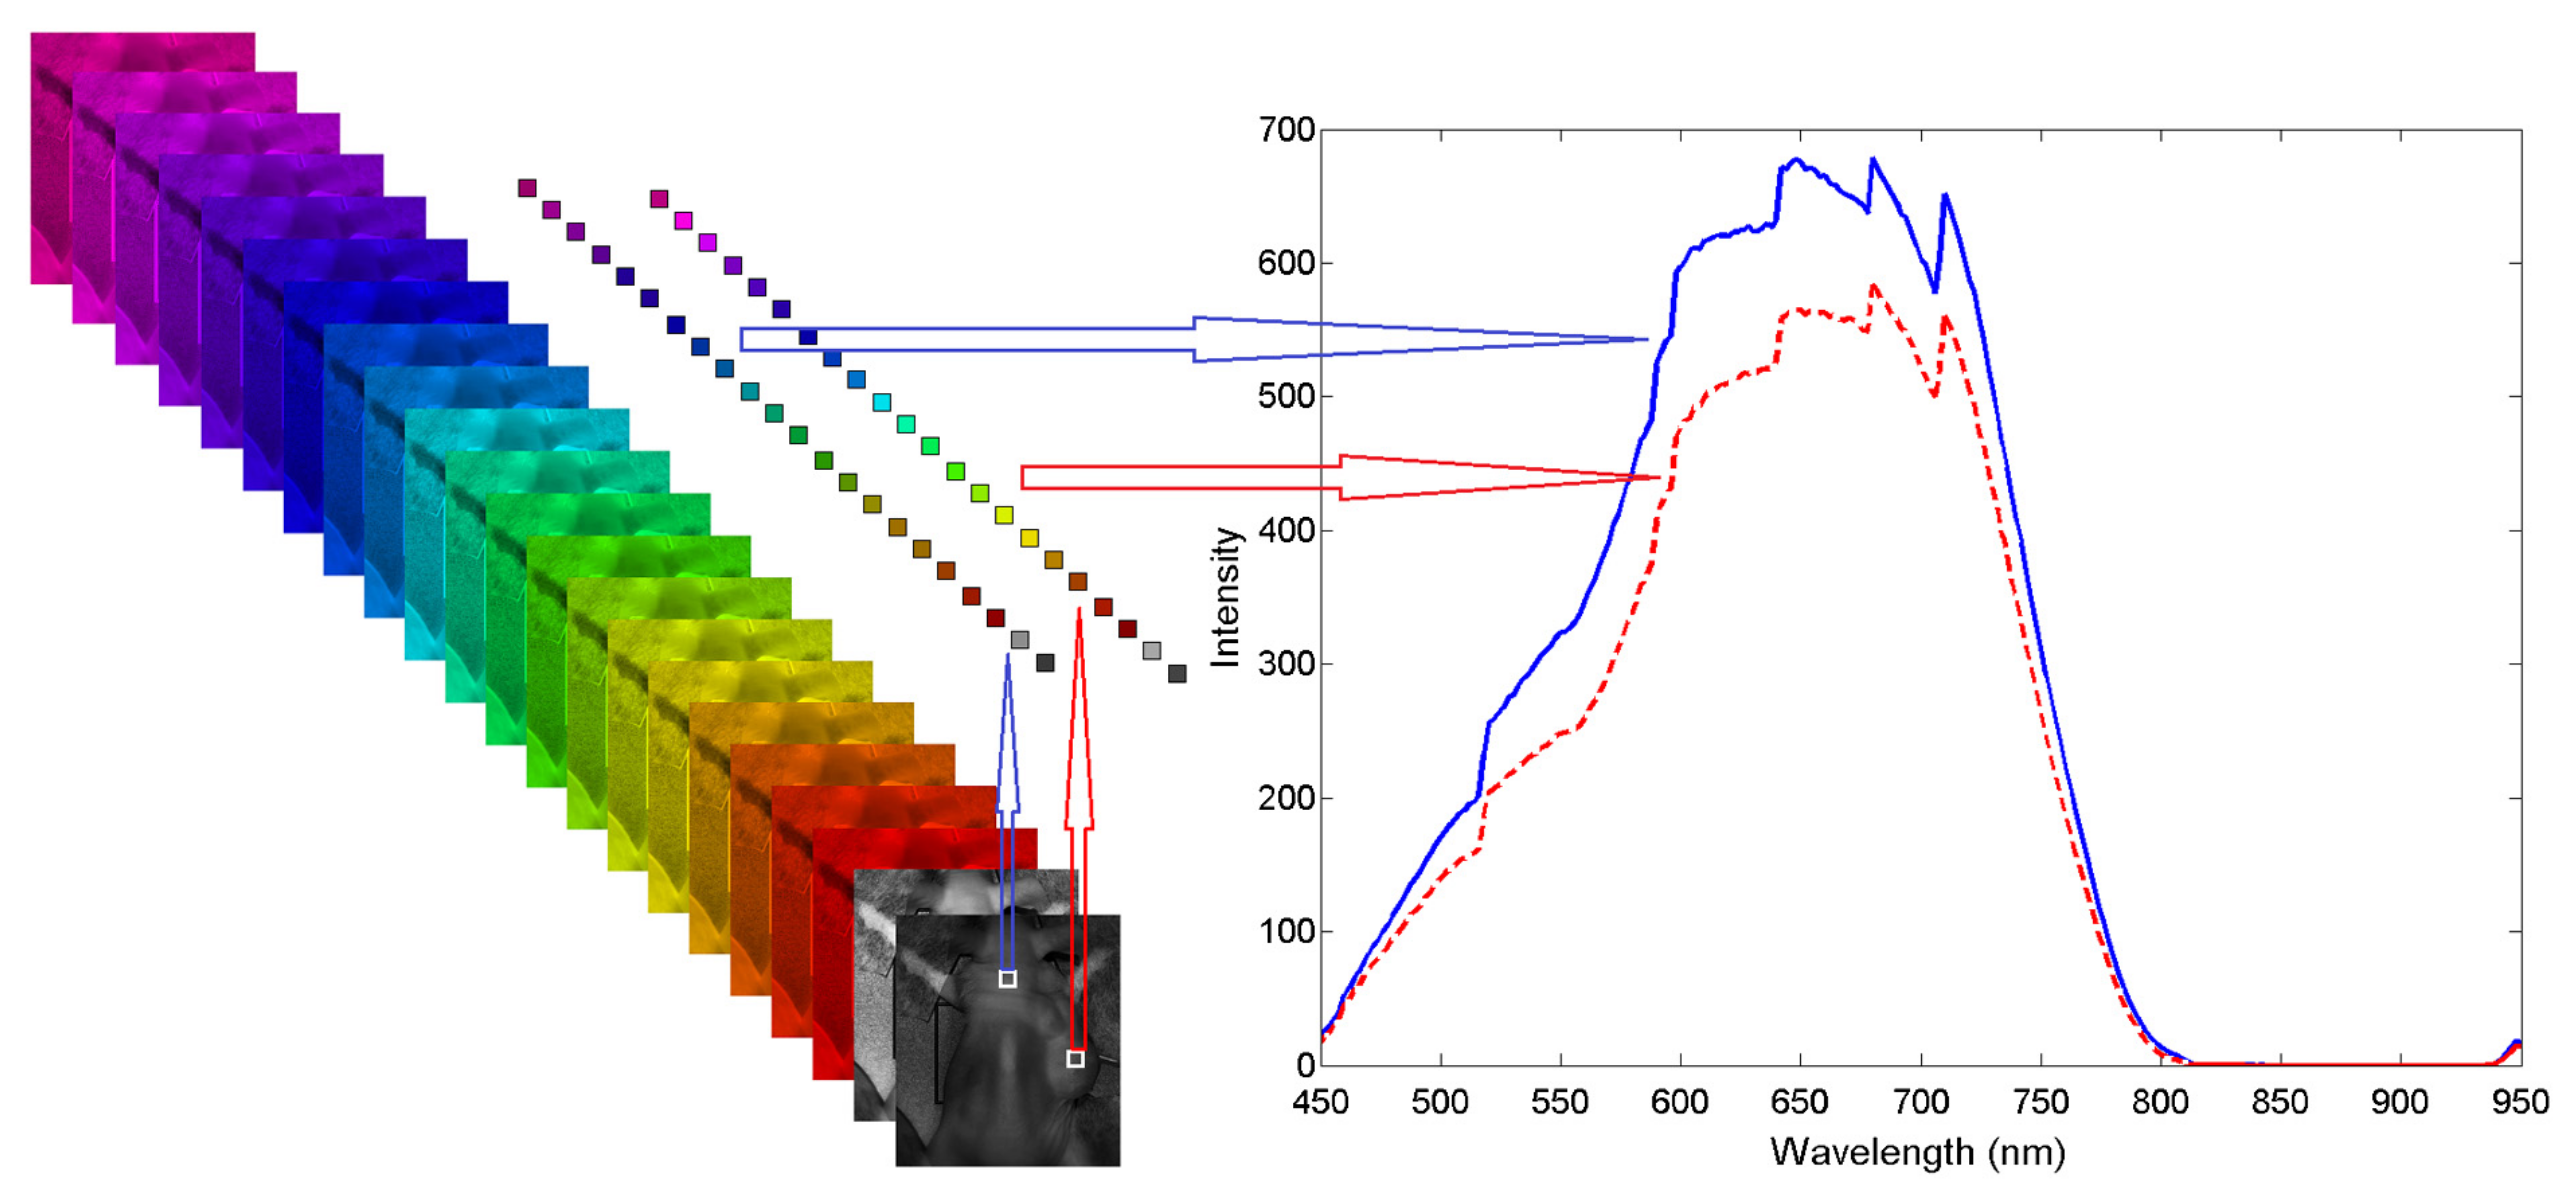
\includegraphics[width=0.61\linewidth]{akabari_figure.png}
    \captionsetup{labelformat=simple, labelsep=colon, font=tiny, labelfont={color=gray,bf}}
    \caption{\textbf{Hyperspectral Images of a Nude Mouse} The left side shows the hyperspectral image cube, while the right side presents spectral graphs of cancer (dashed line) and normal (solid line) tissue, depicting normalized reflectance across wavelengths.)\cite{akbariHyperspectralImagingQuantitative2012}}
    \label{fig:akabari_figure}
\end{figure}
\vspace{-0.3cm}
\begin{itemize}
    \item Akbari, H., Halig, L. V., Schuster, D. M., Osunkoya, A., Master, V., Nieh, P. T., Chen, G. Z., \& Fei, B. (2012). Hyperspectral Imaging and Quantitative Analysis for Prostate Cancer Detection. \textit{Journal of Biomedical Optics}, 17(7), 076005. \href{https://doi.org/10.1117/1.JBO.17.7.076005}{\color{blue}{DOI: 10.1117/1.JBO.17.7.076005}}. \cite{akbariHyperspectralImagingQuantitative2012}
    
    {\color{gray}Describes the use of hyperspectral imaging (HSI) for detecting prostate cancer, highlighting the effectiveness of least squares support vector machines (LS-SVM) in classifying cancerous and normal tissue based on spectral signatures, with reported sensitivity and specificity values of 92.8\% and 96.9\%, respectively.}
    \begin{itemize} \tiny
    \item \textbf{Least Squares Support Vector Machine (LS-SVM):}
    \(
    y(x) = \text{sign} \left( \sum_{k=1}^{N} \alpha_k y_k \Psi(x, x_k) + b \right)
    \)
    
    where \( \alpha_k \) are positive real constants, \( b \) is a real constant, and \( \Psi(x, x_k) = \exp \left( -\frac{\| x - x_k \|^2}{2\sigma^2} \right) \) is the radial basis function kernel.

    \item \textbf{Reflectance Calculation:}
    \(
    R(\lambda) = \frac{I_{\text{raw}}(\lambda) - I_{\text{dark}}(\lambda)}{I_{\text{white}}(\lambda) - I_{\text{dark}}(\lambda)}
    \)
    
    where \( R(\lambda) \) is the reflectance value at wavelength \( \lambda \), \( I_{\text{raw}}(\lambda) \) is the raw radiance value, \( I_{\text{dark}}(\lambda) \) is the dark current radiance, and \( I_{\text{white}}(\lambda) \) is the radiance of the white reference board.

    \item \textbf{Sensitivity and Specificity:}
    \(
    \text{Sensitivity} = \frac{\text{TP}}{\text{TP} + \text{FN}}, \quad \text{Specificity} = \frac{\text{TN}}{\text{TN} + \text{FP}}
    \)
    
    where \( \text{TP} \) and \( \text{FN} \) are true positive and false negative counts, respectively, and \( \text{TN} \) and \( \text{FP} \) are true negative and false positive counts, respectively.
    \end{itemize}

\end{itemize}
\end{frame}
\begin{frame}{}
\tiny
\begin{itemize}
    
    \item Calin, M. A., Parasca, S. V., Savastru, D., \& Manea, D. (2014). Hyperspectral Imaging in the Medical Field: Present and Future. \textit{Applied Spectroscopy Reviews}, 49(6), 435-447. \href{https://doi.org/10.1080/05704928.2013.838678}{\color{blue}{DOI: 10.1080/05704928.2013.838678}}. \cite{calinHyperspectralImagingMedical2014}
    
    {\color{gray}Reviews the current state and future prospects of hyperspectral imaging in medical applications, particularly in disease diagnosis and therapeutic monitoring.}
    \begin{itemize} \tiny
    \item \textbf{Cancer Detection:} Hyperspectral imaging (HSI) is used to detect various types of cancer. The sensitivity and specificity are calculated using the confusion matrix. For example, for gastric cancer: sensitivity = 93\%, specificity = 91\%.
    \item \textbf{Diabetic Foot Ulcers:} HSI measures tissue oxygenation (oxyhemoglobin and deoxyhemoglobin) to predict ulcer healing. The healing prediction index is derived using logistic regression: \[ P(\text{healing}) = \frac{1}{1 + e^{-(a + b_1 \cdot \text{oxy} + b_2 \cdot \text{deoxy})}} \].
    \item \textbf{Tissue Oxygenation:} Uses the modified Beer-Lambert law to produce maps of oxyhemoglobin and deoxyhemoglobin concentrations: \[ A(\lambda) = \log_{10}\left(\frac{I_0(\lambda)}{I(\lambda)}\right) = \epsilon(\lambda) c L \], where \( A(\lambda) \) is absorbance, \( \epsilon(\lambda) \) is the molar absorptivity, \( c \) is the concentration, and \( L \) is the path length.
    
\end{itemize}

\end{itemize}
\end{frame}
\begin{frame}{}
\tiny
\begin{itemize}
    
    \item Schellinger, P.D., et al. (1999). Standardized Stroke MRI: Comparison of Hyperacute Stroke Imaging Protocols. \textit{Stroke}, 30(4), 765-768. \href{https://consensus.app/papers/standardized-stroke-comparison-hemorrhage-schellinger/8fbc8c749c435c8e94e7af9de90a78aa/?utm_source=chatgpt}{\color{blue}{DOI: 10.1161/01.STR.30.4.765}} \cite{tongStandardizedMRIStroke1999}

    {\color{gray}Explores the effectiveness of MRI with hyperspectral imaging for assessing hyperacute intracerebral hemorrhage (ICH) and ischemic strokes.}
    \begin{itemize} \tiny
    \item \textbf{MRI Sensitivity and Specificity:}
    \[
    \text{Sensitivity} = \frac{\text{TP}}{\text{TP} + \text{FN}}, \quad \text{Specificity} = \frac{\text{TN}}{\text{TN} + \text{FP}}
    \]
    where TP is true positive, FN is false negative, TN is true negative, and FP is false positive.
    \item \textbf{Likelihood Ratios:}
    \[
    \text{LR}^+ = \frac{\text{Sensitivity}}{1 - \text{Specificity}}, \quad \text{LR}^- = \frac{1 - \text{Sensitivity}}{\text{Specificity}}
    \]
    where \( \text{LR}^+ \) is the positive likelihood ratio and \( \text{LR}^- \) is the negative likelihood ratio.
    \item \textbf{Confidence Interval for Proportions:}
    \[
    \hat{p} \pm Z \sqrt{\frac{\hat{p}(1 - \hat{p})}{n}}
    \]
    where \( \hat{p} \) is the sample proportion, \( Z \) is the Z-score, and \( n \) is the sample size.
    \item \textbf{Receiver Operating Characteristic (ROC) Curve:}
    \[
    \text{AUC} = \int_{0}^{1} \text{TPR}(FPR) \, d(\text{FPR})
    \]
    where AUC is the area under the curve, TPR is the true positive rate, and FPR is the false positive rate.
    \end{itemize}

\end{itemize}
\end{frame}
\begin{frame}{}
\tiny
\begin{itemize}

    \item Fiebach, J.B., et al. (2004). Stroke Magnetic Resonance Imaging is Accurate in Hyperacute Stroke: A Cohort Study. \textit{Stroke}, 35(2), 502-506. \href{https://consensus.app/papers/stroke-magnetic-resonance-imaging-accurate-hyperacute-fiebach/f5f34a7ddc415e8b88f3c4b51ee76d5c/?utm_source=chatgpt}{\color{blue}{DOI: 10.1161/01.STR.0000114871.19735.23}} \cite{fiebachStrokeMagneticResonance2004}

    {\color{gray}Investigates the accuracy of MRI with hyperspectral imaging in diagnosing hyperacute strokes.}
    \begin{itemize} \tiny
    \item \textbf{Sensitivity and Specificity:}
    \[
    \text{Sensitivity} = \frac{\text{TP}}{\text{TP} + \text{FN}}, \quad \text{Specificity} = \frac{\text{TN}}{\text{TN} + \text{FP}}
    \]
    where TP is true positive, FN is false negative, TN is true negative, and FP is false positive.
    \item \textbf{Positive and Negative Predictive Values:}
    \[
    \text{PPV} = \frac{\text{TP}}{\text{TP} + \text{FP}}, \quad \text{NPV} = \frac{\text{TN}}{\text{TN} + \text{FN}}
    \]
    where PPV is positive predictive value and NPV is negative predictive value.
    \item \textbf{Confidence Interval (CI) for Sensitivity:}
    \[
    \text{CI} = \hat{p} \pm Z \sqrt{\frac{\hat{p}(1 - \hat{p})}{n}}
    \]
    where \( \hat{p} \) is the sample proportion, \( Z \) is the Z-score, and \( n \) is the sample size.
    \item \textbf{Spearman's Signed-Rank Correlation:}
    \[
    r_s = 1 - \frac{6 \sum d_i^2}{n(n^2 - 1)}
    \]
    where \( d_i \) is the difference between the ranks of each observation and \( n \) is the number of observations.
    \end{itemize}

\end{itemize}
\end{frame}
\begin{frame}
\tiny
\begin{itemize}

    \item Ortega, S., Fabelo, H., Camacho, R., Plaza, M. L., Callicó, G. M., \& Sarmiento, R. (2018). Detecting brain tumor in pathological slides using hyperspectral imaging. \textit{Biomedical Optics Express}, 9(2), 818-831. \href{https://doi.org/10.1364/BOE.9.000818}{\color{blue}{DOI: 10.1364/BOE.9.000818}}. \cite{ortegaDetectingBrainTumor2018}

    {\color{gray}Presents a proof-of-concept study using hyperspectral imaging (HSI) data to automatically detect high-grade glioma brain tumors in pathological slides, employing supervised classification algorithms (SVM, ANN, and RF) and demonstrating HSI's suitability for accurate tumor detection.}
    \begin{itemize} \tiny
        \item \textbf{Beer-Lambert Law:}
    \[
    A(\lambda) = \epsilon(\lambda) c d
    \]
    where \( A(\lambda) \) is the absorbance at wavelength \( \lambda \), \( \epsilon(\lambda) \) is the molar absorptivity, \( c \) is the concentration of the absorbing species, and \( d \) is the path length.

    \item \textbf{Support Vector Machine (SVM):}
    \[
    \min_{\mathbf{w}, b, \xi} \frac{1}{2} \|\mathbf{w}\|^2 + C \sum_{i=1}^n \xi_i
    \]
    subject to \( y_i (\mathbf{w}^T \phi(\mathbf{x}_i) + b) \geq 1 - \xi_i \) and \( \xi_i \geq 0 \), where \( C \) is the penalty parameter, \( \phi(\cdot) \) is the kernel function, and \( \xi_i \) are slack variables.

    \item \textbf{Artificial Neural Network (ANN):}
    \[
    y = \sigma(\mathbf{W}^T \mathbf{x} + b)
    \]
    where \( y \) is the output, \( \sigma \) is the activation function, \( \mathbf{W} \) is the weight matrix, \( \mathbf{x} \) is the input vector, and \( b \) is the bias term.

    \item \textbf{Random Forest (RF):}
    \[
    \hat{y} = \frac{1}{N} \sum_{i=1}^N f_i(\mathbf{x})
    \]
    where \( \hat{y} \) is the predicted output, \( N \) is the number of trees in the forest, and \( f_i \) is the prediction of the \( i \)-th tree.

    \item \textbf{Overall Accuracy (OA):}
    \[
    \text{OA} = \frac{\text{Total Success}}{\text{Total Population}}
    \]
    \end{itemize}

\end{itemize}
\end{frame}
\begin{frame}{}
\tiny
\begin{itemize}

    \item Ortega, S., Halicek, M., Fabelo, H., Callico, G. M., & Fei, B. (2020). Hyperspectral and Multispectral Imaging in Digital and Computational Pathology: A Systematic Review. \textit{Biomedical Optics Express}, 11(6), 3195-3242. \href{https://doi.org/10.1364/BOE.386338}{\color{blue}{DOI: 10.1364/BOE.386338}}. \cite{ortegaHyperspectralMultispectralImaging2020}

    {\color{gray}This systematic review summarizes the methods and uses of hyperspectral and multispectral imaging (HSI/MSI) for various pathological applications, including staining and color correction, immunohistochemistry, autofluorescence, and histopathological diagnostic research. It highlights the potential improvements in disease detection and clinical practice offered by HSI/MSI compared to traditional RGB analysis.}
    \begin{itemize} \tiny
    \item \textbf{Beer-Lambert Law:}
    \[
    A(\lambda) = \epsilon(\lambda) c d
    \]
    where \( A(\lambda) \) is the absorbance at wavelength \( \lambda \), \( \epsilon(\lambda) \) is the molar absorptivity, \( c \) is the concentration of the absorbing species, and \( d \) is the path length.

    \item \textbf{Principal Component Analysis (PCA):}
    \[
    \mathbf{X} = \mathbf{TP}^T + \mathbf{E}
    \]
    where \( \mathbf{X} \) is the data matrix, \( \mathbf{T} \) are the scores, \( \mathbf{P} \) are the loadings, and \( \mathbf{E} \) is the residual matrix.

    \item \textbf{Support Vector Machine (SVM):}
    \[
    \min_{\mathbf{w}, b, \xi} \frac{1}{2} \|\mathbf{w}\|^2 + C \sum_{i=1}^n \xi_i
    \]
    subject to \( y_i (\mathbf{w}^T \phi(\mathbf{x}_i) + b) \geq 1 - \xi_i \) and \( \xi_i \geq 0 \), where \( C \) is the penalty parameter, \( \phi(\cdot) \) is the kernel function, and \( \xi_i \) are slack variables.

    \item \textbf{Mutual Information:}
    \[
    I(X;Y) = \sum_{y \in Y} \sum_{x \in X} p(x, y) \log \frac{p(x, y)}{p(x)p(y)}
    \]
    where \( I(X; Y) \) is the mutual information between \( X \) and \( Y \), and \( p(x, y) \) is the joint probability distribution of \( X \) and \( Y \).

    \item \textbf{Normalized Difference Index (NDI):}
    \[
    NDI = \frac{\rho_{X} - \rho_{Y}}{\rho_{X} + \rho_{Y}}
    \]
    where \( \rho_{X} \) and \( \rho_{Y} \) are the reflectances at two different wavelengths.
    \end{itemize}

\end{itemize}
\end{frame}
\begin{frame}
\tiny
\begin{itemize}

    \item Lu, G., Fei, B. (2014). Medical Hyperspectral Imaging: A Review. \textit{Journal of Biomedical Optics}, 19(1), 010901. \href{https://www.spiedigitallibrary.org/journals/journal-of-biomedical-optics/volume-19/issue-01/010901/Medical-hyperspectral-imaging-a-review/10.1117/1.JBO.19.1.010901.full}{\color{blue}{DOI: 10.1117/1.JBO.19.1.010901}} \cite{luMedicalHyperspectralImaging2014}
    
    {\color{gray}Reviews the applications of hyperspectral imaging in medical fields, particularly in disease diagnosis and image-guided surgery.}
    \begin{itemize} \tiny
    \item \textbf{Tissue Optics:}
    \begin{itemize} \tiny
        \item \textbf{Beer-Lambert Law:}
        \[
        A(\lambda) = \log_{10}\left(\frac{I_0(\lambda)}{I(\lambda)}\right) = \epsilon(\lambda) c L
        \]
        where \(A(\lambda)\) is absorbance, \(I_0(\lambda)\) is the incident light intensity, \(I(\lambda)\) is the transmitted light intensity, \(\epsilon(\lambda)\) is the molar absorptivity, \(c\) is the concentration, and \(L\) is the path length.
        \item \textbf{Light Scattering:} Described using Mie and Rayleigh scattering models.
        \[
        \text{Scattering Coefficient} = \frac{24\pi^3 r^6}{\lambda^4} \left(\frac{n^2-1}{n^2+2}\right)^2
        \]
        where \(r\) is the particle radius, \(\lambda\) is the wavelength, and \(n\) is the refractive index.
    \end{itemize}
    \item \textbf{Fluorescence:} Fluorescence intensity \(I_f\) is proportional to the concentration of fluorophores \(c_f\) and the quantum yield \(\Phi\):
    \[
    I_f \propto c_f \Phi I_0
    \]
    where \(I_0\) is the incident light intensity.
    \item \textbf{Principal Component Analysis (PCA):} Dimensionality reduction method.
    \[
    \mathbf{X} = \mathbf{TP}^T + \mathbf{E}
    \]
    where \(\mathbf{X}\) is the data matrix, \(\mathbf{T}\) are the scores, \(\mathbf{P}\) are the loadings, and \(\mathbf{E}\) is the residual matrix.
    \item \textbf{Support Vector Machines (SVM):} Classification method.
    \[
    f(x) = \sum_{i=1}^{n} \alpha_i y_i K(x_i, x) + b
    \]
    where \(\alpha_i\) are the Lagrange multipliers, \(y_i\) are the class labels, \(K\) is the kernel function, and \(b\) is the bias term.
    \item \textbf{Spectral Angle Mapper (SAM):} Measures the spectral similarity between two spectra.
    \[
    \theta = \cos^{-1} \left(\frac{\mathbf{t} \cdot \mathbf{r}}{\|\mathbf{t}\| \|\mathbf{r}\|}\right)
    \]
    where \(\mathbf{t}\) is the target spectrum, and \(\mathbf{r}\) is the reference spectrum.
    \end{itemize}

\end{itemize}
\end{frame}
\begin{frame}{}
\tiny
\begin{itemize}

    \item Fei, B. (2019). Hyperspectral Imaging in Medical Applications. In Q. Liu \& Y. Li (Eds.), \textit{Hyperspectral Imaging} (pp. 523-550). Elsevier. \href{https://doi.org/10.1016/B978-0-444-63977-6.00021-3}{\color{blue}{DOI: 10.1016/B978-0-444-63977-6.00021-3}} \cite{feiHyperspectralImagingMedical2019}
    
    {\color{gray}Explores the applications of hyperspectral imaging in the medical field, emphasizing its potential for noninvasive disease diagnosis and surgical guidance.}
    \begin{itemize} \tiny
    \item \textbf{Oxyhemoglobin and Deoxyhemoglobin Measurements:} Uses the Beer-Lambert law for tissue oxygenation.
    \[
    A(\lambda) = \epsilon_{\text{HbO}_2}(\lambda) c_{\text{HbO}_2} + \epsilon_{\text{Hb}}(\lambda) c_{\text{Hb}}
    \]
    Where \( A(\lambda) \) is the absorbance, \( \epsilon \) are the molar absorptivity coefficients, and \( c \) are the concentrations.
    \item \textbf{Principal Component Analysis (PCA):} Reduces dimensionality in hyperspectral data.
    \[
    \mathbf{X} = \mathbf{TP}^T + \mathbf{E}
    \]
    Where \( \mathbf{X} \) is the data matrix, \( \mathbf{T} \) are the scores, \( \mathbf{P} \) are the loadings, and \( \mathbf{E} \) is the residual matrix.
    \end{itemize}

\end{itemize}
\end{frame}
\begin{frame}
\tiny
\begin{itemize}

    \item Lu, B., Dao, P.D., Liu, J., et al. (2020). Recent Advances of Hyperspectral Imaging Technology and Applications in Agriculture. \textit{Remote Sensing}, 12(15), 2659. \href{https://doi.org/10.3390/rs12162659}{\color{blue}{DOI: 10.3390/rs12152659}} \cite{luRecentAdvancesHyperspectral2020}
    
    {\color{gray}Reviews recent advancements in hyperspectral imaging technology and its applications in agriculture, discussing mini-sized and low-cost airborne hyperspectral sensors.}
    \begin{itemize} \tiny
    \item \textbf{Support Vector Machines (SVM):} SVM classifiers are used with kernel functions to handle the high-dimensional hyperspectral data. The classification function is given by: \[ f(x) = \sum_{i=1}^{n} \alpha_i K(x, x_i) + b \], where \( K \) is the kernel function.
    \item \textbf{Markov Random Fields (MRF):} MRF models the spatial dependencies between pixels. The energy function to be minimized is: \[ E(x) = \sum_{i} U(x_i) + \sum_{i,j} V(x_i, x_j) \], where \( U \) is the unary potential and \( V \) is the pairwise potential.
    \item \textbf{Morphological Processing:} Uses mathematical morphology for feature extraction. The extended morphological profiles (EMP) are constructed by applying morphological operators to hyperspectral data.
    \end{itemize}













\end{itemize}
\end{frame}
\begin{frame}{}
\tiny
\vspace{-0.18cm}
\begin{figure}
    \centering
    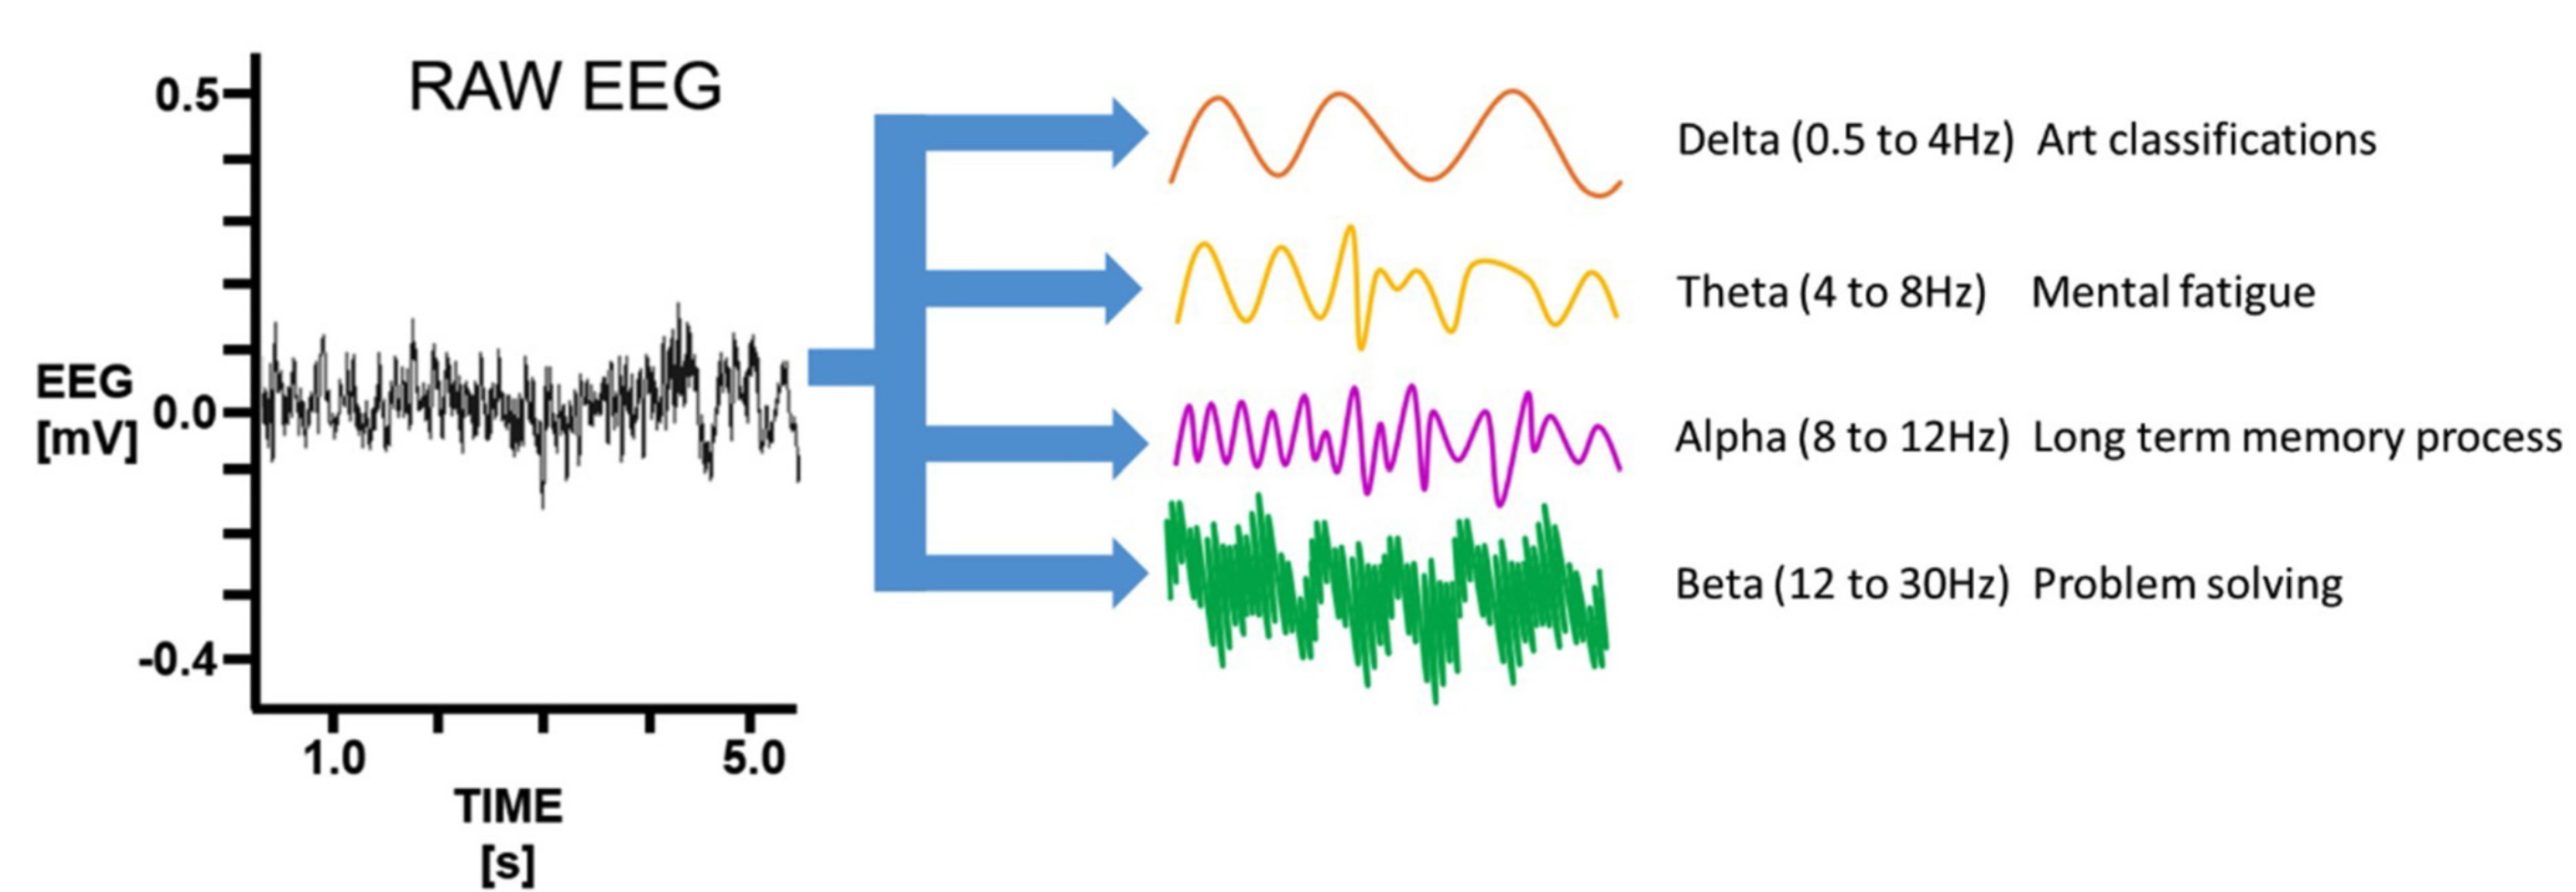
\includegraphics[width=0.62\linewidth]{robotor_figure.png}
    \captionsetup{labelformat=simple, labelsep=colon, font=tiny, labelfont={color=gray,bf}}
    \caption{\textbf{EEG Frequency Bands and Brain Activity} The schematic shows the raw EEG trace decomposed into delta (0.5 to 4 Hz), theta (4 to 8 Hz), alpha (8 to 12 Hz), and beta (12 to 30 Hz) waves, each associated with different brain functions such as art classification, mental fatigue, memory processing, and problem solving.)\cite{portillo-laraMindGapStateoftheart2021}}
    \label{fig:robotor_figure}
\end{figure}
\vspace{-0.2cm} % Adjust this value as needed to reduce the space
\begin{itemize}
    \item Portillo-Lara, R., Tahirbegi, B., Chapman, C. A. R., Goding, J. A., \& Green, R. A. (2021). Mind the gap: State-of-the-art technologies and applications for EEG-based brain–computer interfaces. \textit{APL Bioengineering}, 5, 031507. \href{https://doi.org/10.1063/5.0047237}{\color{blue}{DOI: 10.1063/5.0047237}}. \cite{portillo-laraMindGapStateoftheart2021}

    {\color{gray}Reviews the state-of-the-art technologies and applications for EEG-based brain–computer interfaces (eBCIs), focusing on wearable biosensing, commercial EEG platforms, emerging applications, and ethical, social, and legal concerns associated with eBCI technology.}
    \begin{itemize} \tiny
    \item \textbf{Information Transfer Rate (ITR):}
    \(
    \text{ITR} = \left\{ \log_2 N + P \log_2 P + (1 - P) \log_2 \left( \frac{1 - P}{N - 1} \right) \right\} \cdot \frac{60}{T}
    \)
    
    where \( N \) is the number of possible targets, \( P \) is the accuracy, and \( T \) is the time in seconds.

    \item \textbf{Linear Discriminant Analysis (LDA):}
    \(
    y = \arg\max_k \left( \mathbf{w}_k^T \mathbf{x} + b_k \right)
    \)
    
    where \( \mathbf{w}_k \) is the weight vector, \( \mathbf{x} \) is the feature vector, and \( b_k \) is the bias term for class \( k \).

    \item \textbf{Mutual Information:}
    \(
    I(X;Y) = \sum_{y \in Y} \sum_{x \in X} p(x, y) \log \frac{p(x, y)}{p(x)p(y)}
    \)
    
    where \( I(X; Y) \) is the mutual information between \( X \) and \( Y \), and \( p(x, y) \) is the joint probability distribution of \( X \) and \( Y \).

    \item \textbf{Pearson Correlation Coefficient:}
    \(
    \rho_{X,Y} = \frac{\text{cov}(X, Y)}{\sigma_X \sigma_Y}
    \)
    
    where \( \rho_{X,Y} \) is the Pearson correlation coefficient, \( \text{cov}(X, Y) \) is the covariance of \( X \) and \( Y \), and \( \sigma_X \) and \( \sigma_Y \) are the standard deviations of \( X \) and \( Y \), respectively.
    \end{itemize}

\end{itemize}
\end{frame}
\begin{frame}
\tiny
\begin{itemize}
    
    \item Ahn, S., & Jun, S. C. (2017). Multi-Modal Integration of EEG-fNIRS for Brain-Computer Interfaces – Current Limitations and Future Directions. \textit{Frontiers in Human Neuroscience}, 11:503. \href{https://doi.org/10.3389/fnhum.2017.00503}{\color{blue}{DOI: 10.3389/fnhum.2017.00503}}. \cite{ahnMultiModalIntegrationEEGfNIRS2017}

    {\color{gray}Reviews the current limitations and future directions of integrating electroencephalography (EEG) and functional near-infrared spectroscopy (fNIRS) for brain-computer interfaces (BCIs), discussing the potential benefits and challenges associated with multi-modal integration to enhance BCI performance.}
    \begin{itemize} \tiny
    \item \textbf{Pearson Correlation Coefficient:}
    \[
    \rho_{X,Y} = \frac{\text{cov}(X, Y)}{\sigma_X \sigma_Y}
    \]
    where \( \rho_{X,Y} \) is the Pearson correlation coefficient, \( \text{cov}(X, Y) \) is the covariance of \( X \) and \( Y \), and \( \sigma_X \) and \( \sigma_Y \) are the standard deviations of \( X \) and \( Y \), respectively.

    \item \textbf{Linear Discriminant Analysis (LDA):}
    \[
    y = \arg\max_k \left( \mathbf{w}_k^T \mathbf{x} + b_k \right)
    \]
    where \( \mathbf{w}_k \) is the weight vector, \( \mathbf{x} \) is the feature vector, and \( b_k \) is the bias term for class \( k \).

    \item \textbf{Modified Beer-Lambert Law:}
    \[
    A(\lambda) = \epsilon(\lambda) c d
    \]
    where \( A(\lambda) \) is the absorbance at wavelength \( \lambda \), \( \epsilon(\lambda) \) is the molar absorptivity, \( c \) is the concentration of the absorbing species, and \( d \) is the path length.

    \item \textbf{Mutual Information:}
    \[
    I(X;Y) = \sum_{y \in Y} \sum_{x \in X} p(x, y) \log \frac{p(x, y)}{p(x)p(y)}
    \]
    where \( I(X; Y) \) is the mutual information between \( X \) and \( Y \), and \( p(x, y) \) is the joint probability distribution of \( X \) and \( Y \).
    
    \item \textbf{Receiver Operating Characteristic (ROC) Curve:}
    \[
    \text{AUC} = \int_{0}^{1} \text{TPR}(\text{FPR}) \, d(\text{FPR})
    \]
    where AUC is the area under the ROC curve, TPR is the true positive rate, and FPR is the false positive rate.
\end{itemize}
    

\end{itemize}
\end{frame}
\begin{frame}
\tiny
\begin{itemize}

    \item Hasan, M. A. H., Khan, M. U., \& Mishra, D. (2020). A Computationally Efficient Method for Hybrid EEG-fNIRS BCI Based on the Pearson Correlation. \textit{BioMed Research International}, 2020, Article ID 1838140, 13 pages. \href{https://doi.org/10.1155/2020/1838140}{\color{blue}{DOI: 10.1155/2020/1838140}}. \cite{hasanComputationallyEfficientMethod2020}

    {\color{gray}Proposes a novel channel selection approach for hybrid EEG-fNIRS BCI systems using the Pearson product-moment correlation coefficient to select highly correlated channels, demonstrating significant reduction in computational burden while maintaining high classification accuracy.}
    \begin{itemize} \tiny
    \item \textbf{Pearson Product-Moment Correlation Coefficient (PPMCC):}
    \[
    \rho_{i,j} = \frac{E[(X_i - \mu_i)(X_j - \mu_j)]}{\sigma_i \sigma_j}
    \]
    where \( \rho_{i,j} \) is the correlation coefficient between channels \( i \) and \( j \), \( \mu \) is the mean value, \( \sigma \) is the standard deviation, and \( E \) is the expectation operator.

    \item \textbf{Signal Mean (M):}
    \[
    M = \frac{1}{N} \sum_{i=1}^{N} X_i
    \]
    where \( M \) is the mean value of the signal, \( X \) is the signal, and \( N \) is the total number of observations.

    \item \textbf{Signal Skewness (SK):}
    \[
    SK(X) = E\left[\left(\frac{X - \mu}{\sigma}\right)^3\right]
    \]
    where \( SK \) is the skewness of the signal, \( \mu \) is the mean, and \( \sigma \) is the standard deviation.

    \item \textbf{Signal Kurtosis (KR):}
    \[
    KR(X) = E\left[\left(\frac{X - \mu}{\sigma}\right)^4\right]
    \]
    where \( KR \) is the kurtosis of the signal, \( \mu \) is the mean, and \( \sigma \) is the standard deviation.

    \item \textbf{Signal Peak (P):}
    \[
    P = \max(X_i)
    \]
    where \( P \) is the peak value of the signal.
    \end{itemize}
    
\end{itemize}
\end{frame}
\begin{frame}
\tiny
\begin{itemize}

    \item Corsi, M.-C., Chavez, M., Schwartz, D., Hugueville, L., Khambhati, A. N., Bassett, D. S., & De Vico Fallani, F. (2018). Integrating EEG and MEG Signals to Improve Motor Imagery Classification in Brain-Computer Interface. \textit{arXiv}, 1711.07258. \href{https://arxiv.org/abs/1711.07258}{\color{blue}{arXiv:1711.07258}}. \cite{corsiIntegratingEEGMEG2018}
    
    {\color{gray}Proposes a fusion approach that combines features from electroencephalographic (EEG) and magnetoencephalographic (MEG) signals to enhance classification performance in motor imagery-based brain-computer interfaces (BCIs), demonstrating significant improvements in classification accuracy.}
    \begin{itemize} \tiny
    \item \textbf{Power Spectrum Calculation:}
    \[
    P(f) = \frac{1}{T} \left| \int_{0}^{T} x(t) e^{-j2\pi ft} dt \right|^2
    \]
    where \( P(f) \) is the power spectrum, \( x(t) \) is the time-domain signal, and \( T \) is the time period.

    \item \textbf{Linear Discriminant Analysis (LDA):}
    \[
    y = \arg\max_k \left( \mathbf{w}_k^T \mathbf{x} + b_k \right)
    \]
    where \( \mathbf{w}_k \) is the weight vector, \( \mathbf{x} \) is the feature vector, and \( b_k \) is the bias term for class \( k \).

    \item \textbf{Bayesian Fusion Approach:}
    \[
    \lambda_i = \frac{p_i}{p_{\text{EEG}} + p_{\text{MAG}} + p_{\text{GRAD}}}
    \]
    where \( \lambda_i \) is the weight parameter for modality \( i \), and \( p_i \) is the posterior probability from the classification of modality \( i \).

    \item \textbf{Area Under the Curve (AUC):}
    \[
    \text{AUC} = \int_{0}^{1} \text{TPR}(\text{FPR}) \, d(\text{FPR})
    \]
    where AUC is the area under the receiver operating characteristic (ROC) curve, TPR is the true positive rate, and FPR is the false positive rate.
\end{itemize}










\end{itemize}
\end{frame}
\begin{frame}
\tiny
\begin{itemize}

    \item Khan, U., Paheding, S., Elkin, C. P., \& Devabhaktuni, V. K. (2021). Trends in Deep Learning for Medical Hyperspectral Image Analysis. \textit{IEEE Access}, 9, 79534-79545. \href{https://doi.org/10.1109/ACCESS.2021.3068392}{\color{blue}{DOI: 10.1109/ACCESS.2021.3068392}}. \cite{khanTrendsDeepLearning2021}

    {\color{gray}Reviews the latest trends in deep learning applications for medical hyperspectral imaging, focusing on classification, detection, and segmentation tasks, and discusses current challenges and future directions in this field.}
    \begin{itemize} \tiny
    \item \textbf{Convolutional Neural Network (CNN):}
    \[
    y = f(W * x + b)
    \]
    where \( y \) is the output, \( W \) is the filter, \( x \) is the input, \( b \) is the bias, and \( * \) denotes the convolution operation.
    \item \textbf{Softmax Function:}
    \[
    \text{Softmax}(z_i) = \frac{e^{z_i}}{\sum_{j} e^{z_j}}
    \]
    where \( z_i \) is the input to the \( i \)-th neuron.
    \item \textbf{Cross-Entropy Loss:}
    \[
    L = -\sum_{i} y_i \log(\hat{y}_i)
    \]
    where \( y_i \) is the true label, and \( \hat{y}_i \) is the predicted probability.
    \item \textbf{Autoencoder:}
    \[
    L = \| x - \hat{x} \|^2
    \]
    where \( x \) is the input, and \( \hat{x} \) is the reconstructed input.
    \end{itemize}

\end{itemize}
\end{frame}
\begin{frame}
\tiny
\begin{itemize}

    \item Cui, R., Yu, H., Xu, T., Xing, X., Cao, X., Yan, K., \& Chen, J. (2022). Deep Learning in Medical Hyperspectral Images: A Review. \textit{Sensors}, 22(24), 9790. \href{https://doi.org/10.3390/s22249790}{\color{blue}{DOI: 10.3390/s22249790}}. \cite{cuiDeepLearningMedical2022}

    {\color{gray}Reviews the progress of deep learning in the analysis and recognition of medical hyperspectral images, summarizing common imaging systems, preprocessing techniques, and the main developments in deep learning for disease diagnosis.}
    \begin{itemize} \tiny
    \item \textbf{Normalized Reflectance Calculation:}
    \[
    I_{\text{ref}} = \frac{I_{\text{raw}} - I_{\text{dark}}}{I_{\text{white}} - I_{\text{dark}}}
    \]
    where \( I_{\text{ref}} \) is the normalized reflectance, \( I_{\text{raw}} \) is the raw intensity, \( I_{\text{dark}} \) is the dark reference, and \( I_{\text{white}} \) is the white reference.

    \item \textbf{Standard Normal Variate (SNV):}
    \[
    x_{\text{SNV}} = \frac{x - \bar{x}}{\sqrt{\frac{1}{m-1} \sum_{k=1}^m (x_k - \bar{x})^2}}
    \]
    where \( x \) is the spectral data, \( \bar{x} \) is the mean of \( x \), and \( m \) is the number of wavelength points.

    \item \textbf{Principal Component Analysis (PCA):}
    \[
    \mathbf{X} = \mathbf{U} \mathbf{\Sigma} \mathbf{V}^T
    \]
    where \( \mathbf{X} \) is the data matrix, \( \mathbf{U} \) and \( \mathbf{V} \) are orthogonal matrices, and \( \mathbf{\Sigma} \) is a diagonal matrix of singular values.

    \item \textbf{Convolutional Neural Network (CNN):}
    \[
    y = f(W * x + b)
    \]
    where \( y \) is the output, \( W \) is the filter, \( x \) is the input, \( b \) is the bias, and \( * \) denotes the convolution operation.

    \item \textbf{Softmax Function:}
    \[
    \text{Softmax}(z_i) = \frac{e^{z_i}}{\sum_{j} e^{z_j}}
    \]
    where \( z_i \) is the input to the \( i \)-th neuron.

    \item \textbf{Cross-Entropy Loss:}
    \[
    L = -\sum_{i} y_i \log(\hat{y}_i)
    \]
    where \( y_i \) is the true label, and \( \hat{y}_i \) is the predicted probability.
\end{itemize}

\end{itemize}
\end{frame}
\begin{frame}
\tiny
\begin{itemize}

    \item Yang, X., Ye, Y., Li, X., Lau, R. Y. K., Zhang, X., \& Huang, X. (2018). Hyperspectral Image Classification With Deep Learning Models. \textit{IEEE Transactions on Geoscience and Remote Sensing}, 56(9), 5408-5423. \href{https://doi.org/10.1109/TGRS.2018.2815613}{\color{blue}{DOI: 10.1109/TGRS.2018.2815613}}. \cite{yangHyperspectralImageClassification2018}

    {\color{gray}Proposes deep learning models including 2D-CNN, 3D-CNN, recurrent 2D-CNN (R-2D-CNN), and recurrent 3D-CNN (R-3D-CNN) for hyperspectral image classification, demonstrating their superiority over conventional methods through experiments on multiple data sets.}
    \begin{itemize} \tiny
    \item \textbf{2D-CNN:}
    \(
    v_{i,j}^{xy} = F \left( b_{ij} + \sum_{m} \sum_{p=0}^{N_i-1} \sum_{q=0}^{M_i-1} w_{ijm}^{pq} v_{i-1}^{(x+p)(y+q)} \right)
    \)
    
    where \( v_{i,j}^{xy} \) is the output at position \((x, y)\) of the \(j\)-th feature map at the \(i\)-th layer, \(b_{ij}\) is the bias term, \(F(\cdot)\) is the activation function, and \(w_{ijm}^{pq}\) are the convolution kernel weights.

    \item \textbf{3D-CNN:}
    \(
    v_{i,j}^{xyz} = F \left( b_{ij} + \sum_{m} \sum_{p=0}^{N_i-1} \sum_{q=0}^{M_i-1} \sum_{r=0}^{D_i-1} w_{ijm}^{pqr} v_{i-1}^{(x+p)(y+q)(z+r)} \right)
    \)
    
    where \( v_{i,j}^{xyz} \) is the output at position \((x, y, z)\) of the \(j\)-th feature map at the \(i\)-th layer, and \(D_i\) is the depth of the 3D kernel.

    \item \textbf{Softmax Function:}
    \[
    p(c|I_{i,j,k}; (W, b)) = \frac{e^{f_c(I_{i,j,k}; (W, b))}}{\sum_{d=1}^{N} e^{f_d(I_{i,j,k}; (W, b))}}
    \]
    where \( p(c|I_{i,j,k}; (W, b)) \) is the probability of class \(c\), \( f_c(I_{i,j,k}; (W, b)) \) is the score for class \(c\), and \( (W, b) \) are the parameters.

    \item \textbf{Cross-Entropy Loss:}
    \[
    L(W, b) = - \sum_{I_{i,j,k}} \log p(l_{i,j,k} | I_{i,j,k}; (W, b))
    \]
    where \( l_{i,j,k} \) is the true label of the pixel at position \((i, j)\) of the image \( I_k \).

    \item \textbf{Recurrent 2D-CNN (R-2D-CNN):}
    \[
    F^p = [F(F^{p-1}, I_{i,j,k}^p)], \quad F^1 = [0, I_{i,j,k}^1]
    \]
    where \( F^p \) represents the feature maps at level \(p\), and \( I_{i,j,k}^p \) is the \(p\)-th level instance.
    \end{itemize}
    
\end{itemize}
\end{frame}
\begin{frame}
\tiny
\begin{itemize}

    \item Zhou, X., \& Prasad, S. (2020). Advances in Deep Learning for Hyperspectral Image Analysis – Addressing Challenges Arising in Practical Imaging Scenarios. \textit{arXiv}, 2007.08592. \href{https://arxiv.org/abs/2007.08592}{\color{blue}{arXiv:2007.08592}}. \cite{zhouAdvancesDeepLearning2020}

    {\color{gray}Reviews recent advances in deep learning for hyperspectral image analysis, focusing on challenges such as limited labeled data and high dimensionality, and explores unsupervised, semi-supervised, and transfer learning approaches to address these issues.}
    \begin{itemize} \tiny
    \item \textbf{Unsupervised Feature Learning:}
    \[
    \mathbf{H} = \text{ReLU}(\mathbf{W}_1 \mathbf{X} + \mathbf{b}_1)
    \]
    where \( \mathbf{H} \) is the hidden representation, \( \mathbf{W}_1 \) and \( \mathbf{b}_1 \) are weights and biases, and \(\text{ReLU}\) is the activation function.

    \item \textbf{Semi-Supervised Learning:}
    \[
    L_{\text{semi}} = L_{\text{sup}} + \lambda L_{\text{unsup}}
    \]
    where \( L_{\text{semi}} \) is the total loss, \( L_{\text{sup}} \) is the supervised loss, \( L_{\text{unsup}} \) is the unsupervised loss, and \( \lambda \) is a balancing parameter.

    \item \textbf{Domain Adaptation:}
    \[
    \min_{\mathbf{W}} \left\| \mathbf{W} \mathbf{X}_s - \mathbf{X}_t \right\|^2_F
    \]
    where \( \mathbf{W} \) is the transformation matrix, \( \mathbf{X}_s \) and \( \mathbf{X}_t \) are source and target domain data, and \( \left\| \cdot \right\|_F \) denotes the Frobenius norm.
    \end{itemize}

\end{itemize}
\end{frame}
\begin{frame}
\tiny
\begin{itemize}
    
    \item Wang, C., Liu, B., Liu, L., Zhu, Y., Hou, J., Liu, P., \& Li, X. (2021). A Review of Deep Learning Used in the Hyperspectral Image Analysis for Agriculture. \textit{Artificial Intelligence Review}, 54, 5205-5253. \href{https://doi.org/10.1007/s10462-021-10018-y}{\color{blue}{DOI: 10.1007/s10462-021-10018-y}}. \cite{wangReviewDeepLearning2021}

    {\color{gray}Reviews the application of deep learning techniques in hyperspectral image analysis for agriculture, focusing on the use of convolutional neural networks (CNNs), principal component analysis (PCA), and other deep learning models to improve classification, prediction, and detection tasks in agricultural settings.}
    \begin{itemize} \tiny
    \item \textbf{Convolutional Neural Network (CNN):}
    \[
    v_{i,j}^{xy} = F \left( b_{ij} + \sum_{m} \sum_{p=0}^{N_i-1} \sum_{q=0}^{M_i-1} w_{ijm}^{pq} v_{i-1}^{(x+p)(y+q)} \right)
    \]
    where \( v_{i,j}^{xy} \) is the output at position \((x, y)\) of the \(j\)-th feature map at the \(i\)-th layer, \(b_{ij}\) is the bias term, \(F(\cdot)\) is the activation function, and \(w_{ijm}^{pq}\) are the convolution kernel weights.

    \item \textbf{Principal Component Analysis (PCA):}
    \[
    \mathbf{X} = \mathbf{U} \mathbf{\Sigma} \mathbf{V}^T
    \]
    where \( \mathbf{X} \) is the data matrix, \( \mathbf{U} \) and \( \mathbf{V} \) are orthogonal matrices, and \( \mathbf{\Sigma} \) is a diagonal matrix of singular values.

    \item \textbf{Softmax Function:}
    \[
    \text{Softmax}(z_i) = \frac{e^{z_i}}{\sum_{j} e^{z_j}}
    \]
    where \( z_i \) is the input to the \( i \)-th neuron.

    \item \textbf{Cross-Entropy Loss:}
    \[
    L = -\sum_{i} y_i \log(\hat{y}_i)
    \]
    where \( y_i \) is the true label, and \( \hat{y}_i \) is the predicted probability.
\end{itemize}

\end{itemize}
\end{frame}
\begin{frame}
\tiny
\begin{itemize}

    \item Chen, Y., Jiang, H., Li, C., Jia, X., \& Ghamisi, P. (2016). Deep Feature Extraction and Classification of Hyperspectral Images Based on Convolutional Neural Networks. \textit{IEEE Transactions on Geoscience and Remote Sensing}, 54(10), 6232-6251. \href{https://doi.org/10.1109/TGRS.2016.2584107}{\color{blue}{DOI: 10.1109/TGRS.2016.2584107}}. \cite{chenDeepFeatureExtraction2016}

    {\color{gray}Proposes a 3-D CNN model with combined regularization techniques including L2 regularization and dropout to extract spectral–spatial features from hyperspectral images, and evaluates the model on three widely used hyperspectral datasets.}
    \begin{itemize} \tiny
    \item \textbf{CNN:}
    \(
    v_{i,j}^{xy} = F \left( b_{ij} + \sum_{m} \sum_{p=0}^{N_i-1} \sum_{q=0}^{M_i-1} w_{ijm}^{pq} v_{i-1}^{(x+p)(y+q)} \right)
    \)
    
    where \( v_{i,j}^{xy} \) is the output at position \((x, y)\) of the \(j\)-th feature map at the \(i\)-th layer, \(b_{ij}\) is the bias term, \(F(\cdot)\) is the activation function, and \(w_{ijm}^{pq}\) are the convolution kernel weights.

    \item \textbf{L2 Regularization:}
    \[
    c = c_0 + \frac{\lambda}{2m} \sum_{j=1}^{N} w_j^2
    \]
    where \( c \) is the modified cost function, \( c_0 \) is the original cost, \( \lambda \) is the regularization parameter, \( m \) is the mini-batch size, \( N \) is the number of weights, and \( w_j \) are the weights.

    \item \textbf{Dropout:}
    \[
    \text{Dropout}(h) = \begin{cases} 
    0 & \text{with probability } p \\
    \frac{h}{1-p} & \text{with probability } 1-p 
    \end{cases}
    \]
    where \( h \) is the input to the dropout layer, and \( p \) is the dropout rate.
    
    \item \textbf{Softmax Function:}
    \[
    \text{Softmax}(z_i) = \frac{e^{z_i}}{\sum_{j} e^{z_j}}
    \]
    where \( z_i \) is the input to the \( i \)-th neuron.

    \item \textbf{Cross-Entropy Loss:}
    \[
    L = -\sum_{i} y_i \log(\hat{y}_i)
    \]
    where \( y_i \) is the true label, and \( \hat{y}_i \) is the predicted probability.
\end{itemize}

\end{itemize}
\end{frame}
\begin{frame}
\tiny
\begin{itemize}

    \item Liu, B., Yu, A., Yu, X., Wang, R., Gao, K., \& Guo, W. (2021). Deep Multiview Learning for Hyperspectral Image Classification. \textit{IEEE Transactions on Geoscience and Remote Sensing}, 59(9), 7758-7772. \href{https://doi.org/10.1109/TGRS.2020.3034133}{\color{blue}{DOI: 10.1109/TGRS.2020.3034133}}. \cite{liuDeepMultiviewLearning2021}

     {\color{gray}Proposes a deep multiview learning method to address the small sample problem in hyperspectral image (HSI) classification by constructing two views using PCA, embedding these views into a latent space using a deep residual network, and maximizing agreement between views using contrastive loss.}
     \begin{itemize} \tiny
     \item \textbf{Principal Component Analysis (PCA):}
    \[
    \mathbf{X} = \mathbf{U} \mathbf{\Sigma} \mathbf{V}^T
    \]
    where \( \mathbf{X} \) is the data matrix, \( \mathbf{U} \) and \( \mathbf{V} \) are orthogonal matrices, and \( \mathbf{\Sigma} \) is a diagonal matrix of singular values.

    \item \textbf{Contrastive Loss:}
    \[
    \ell(i, j) = - \log \frac{\exp(\text{sim}(z_i, z_j))}{\sum_{k=1}^{2N} \mathbb{1}_{[k \neq i]} \exp(\text{sim}(z_i, z_k))}
    \]
    where \(\text{sim}(z_i, z_j) = \frac{z_i^T z_j}{\|z_i\| \|z_j\|}\) is the cosine similarity, and \( z_i \) and \( z_j \) are feature representations.

    \item \textbf{Residual Network (ResNet) Block:}
    \[
    y = F(x, \{W_i\}) + x
    \]
    where \( F(x, \{W_i\}) \) represents the residual mapping and \( x \) is the input.

    \item \textbf{Support Vector Machine (SVM):}
    \[
    \min_{\mathbf{w}, b, \xi} \frac{1}{2} \|\mathbf{w}\|^2 + C \sum_{i=1}^n \xi_i
    \]
    subject to \( y_i (\mathbf{w}^T \phi(\mathbf{x}_i) + b) \geq 1 - \xi_i \) and \( \xi_i \geq 0 \), where \( C \) is the penalty parameter, \( \phi(\cdot) \) is the kernel function, and \( \xi_i \) are slack variables.
\end{itemize}
     
\end{itemize}
\end{frame}
\begin{frame}
\tiny
\begin{itemize}

    \item Jiang, J., Zhou, Z., Yin, E., Yu, Y., & Hu, D. (2014). Hybrid Brain-Computer Interface (BCI) based on the EEG and EOG signals. \textit{Bio-Medical Materials and Engineering}, 24(6), 2919-2925. \href{https://doi.org/10.3233/BME-141111}{\color{blue}{DOI: 10.3233/BME-141111}}. \cite{jiangHybridBrainComputerInterface2014}

    {\color{gray}Proposes a hybrid brain-computer interface (BCI) system combining electroencephalogram (EEG) and electrooculograph (EOG) signals to improve accuracy and flexibility in target selection tasks, demonstrating an average accuracy of 89.3\% and a completion time of 2.4 seconds.}
    \begin{itemize} \tiny
    \item \textbf{Information Transfer Rate (ITR):}
    \[
    \text{ITR} = \left\{ \log_2 N + P \log_2 P + (1 - P) \log_2 \left( \frac{1 - P}{N - 1} \right) \right\} \cdot \frac{60}{T}
    \]
    where \( N \) is the number of possible targets, \( P \) is the accuracy, and \( T \) is the time in seconds.

    \item \textbf{Common Spatial Pattern (CSP):}
    \[
    \max_w \frac{w^T \Sigma_1 w}{w^T \Sigma_2 w}
    \]
    where \( w \) is the spatial filter, \( \Sigma_1 \) and \( \Sigma_2 \) are the covariance matrices of two different classes.

    \item \textbf{Linear Discriminant Analysis (LDA):}
    \[
    y = \arg\max_k \left( \mathbf{w}_k^T \mathbf{x} + b_k \right)
    \]
    where \( \mathbf{w}_k \) is the weight vector, \( \mathbf{x} \) is the feature vector, and \( b_k \) is the bias term for class \( k \).

    \item \textbf{Receiver Operating Characteristic (ROC) Analysis:}
    \[
    f = \frac{\text{TPR} - \text{FPR}}{2}
    \]
    where \( \text{TPR} \) is the true positive rate and \( \text{FPR} \) is the false positive rate.
\end{itemize}

\end{itemize}
\end{frame}

\section{Benchmark Datasets}
\begin{frame}{Benchmark Datasets in HSI - Part 1}
\small
\begin{figure}
    \centering
    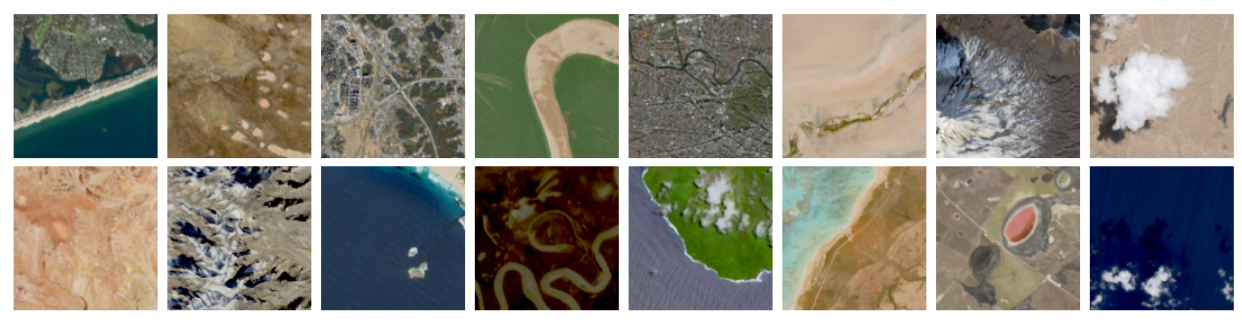
\includegraphics[width=1\linewidth]{HySpecNet_example.png}
    \captionsetup{labelformat=simple, labelsep=colon, font=tiny, labelfont={color=gray,bf}}
    \caption{True color representations of example images from our proposed HySpecNet-11k dataset. Red, green, and blue channels are extracted from EnMAP bands 43, 28, and 10 at wavelengths 634.919 nm, 550.525 nm, and 463.584 nm, respectively.\cite{fuchsHySpecNet11kLargeScaleHyperspectral2023}}
    \label{fig:HySpecNet-example}
\end{figure}
\vspace{-1cm} % Adjust this value as needed to reduce the space
\begin{table}[]
    \centering
    \begin{tabular}{|p{4.5cm}|p{6cm}|p{0.5cm}|}
        \hline
        \textbf{Title (DOI)} & \textbf{Description} & \textbf{Cite} \\ \hline
        HySpecNet-11k: A Large-Scale Hyperspectral Dataset for Image Compression and Unsupervised Learning \newline \href{https://consensus.app/papers/hyspecnet11k-largescale-hyperspectral-dataset-fuchs/86b52e4fcd0c50f6b4c0da950c6e4c11/?utm_source=chatgpt}{\color{blue}10.1109/TGRS.2023.3155567} & This large-scale dataset consists of 11,483 non-overlapping image patches, each with 224 spectral bands, designed for hyperspectral image compression and unsupervised learning tasks. & \cite{fuchsHySpecNet11kLargeScaleHyperspectral2023} \\ \hline
    \end{tabular}
\end{table}
\end{frame}

\begin{frame}{Benchmark Datasets in HSI - Part 1 (Contd.)}
\small
\begin{figure}
    \centering
    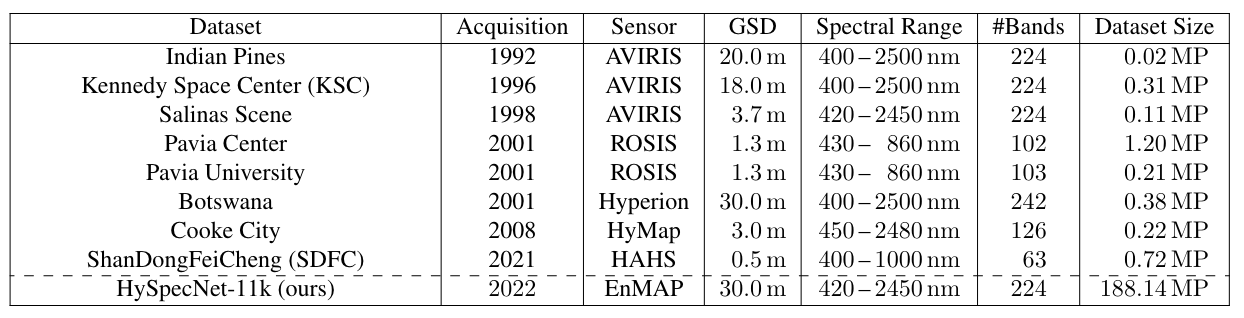
\includegraphics[width=1\linewidth]{HySpecNet_table.png}
    \captionsetup{labelformat=simple, labelsep=colon, font=tiny, labelfont={color=gray,bf}}
    \caption{A summary of publicly available hyperspectral benchmark datasets and their characteristics.\cite{fuchsHySpecNet11kLargeScaleHyperspectral2023}}
    \label{fig:HySpecNet-example}
\end{figure}
\vspace{-0.8cm} % Adjust this value as needed to reduce the space
\begin{table}[]
    \centering
    \begin{tabular}{|p{4.5cm}|p{6cm}|p{0.5cm}|}
        \hline
        \textbf{Title (DOI)} & \textbf{Description} & \textbf{Cite} \\ \hline
        HySpecNet-11k: A Large-Scale Hyperspectral Dataset for Image Compression and Unsupervised Learning \newline \href{https://consensus.app/papers/hyspecnet11k-largescale-hyperspectral-dataset-fuchs/86b52e4fcd0c50f6b4c0da950c6e4c11/?utm_source=chatgpt}{\color{blue}10.1109/TGRS.2023.3155567} & This large-scale dataset consists of 11,483 non-overlapping image patches, each with 224 spectral bands, designed for hyperspectral image compression and unsupervised learning tasks. & \cite{fuchsHySpecNet11kLargeScaleHyperspectral2023} \\ \hline
    \end{tabular}
\end{table}
\end{frame}

\begin{frame}{Benchmark Datasets in HSI - Part 2}
\small
\begin{figure}
    \centering
    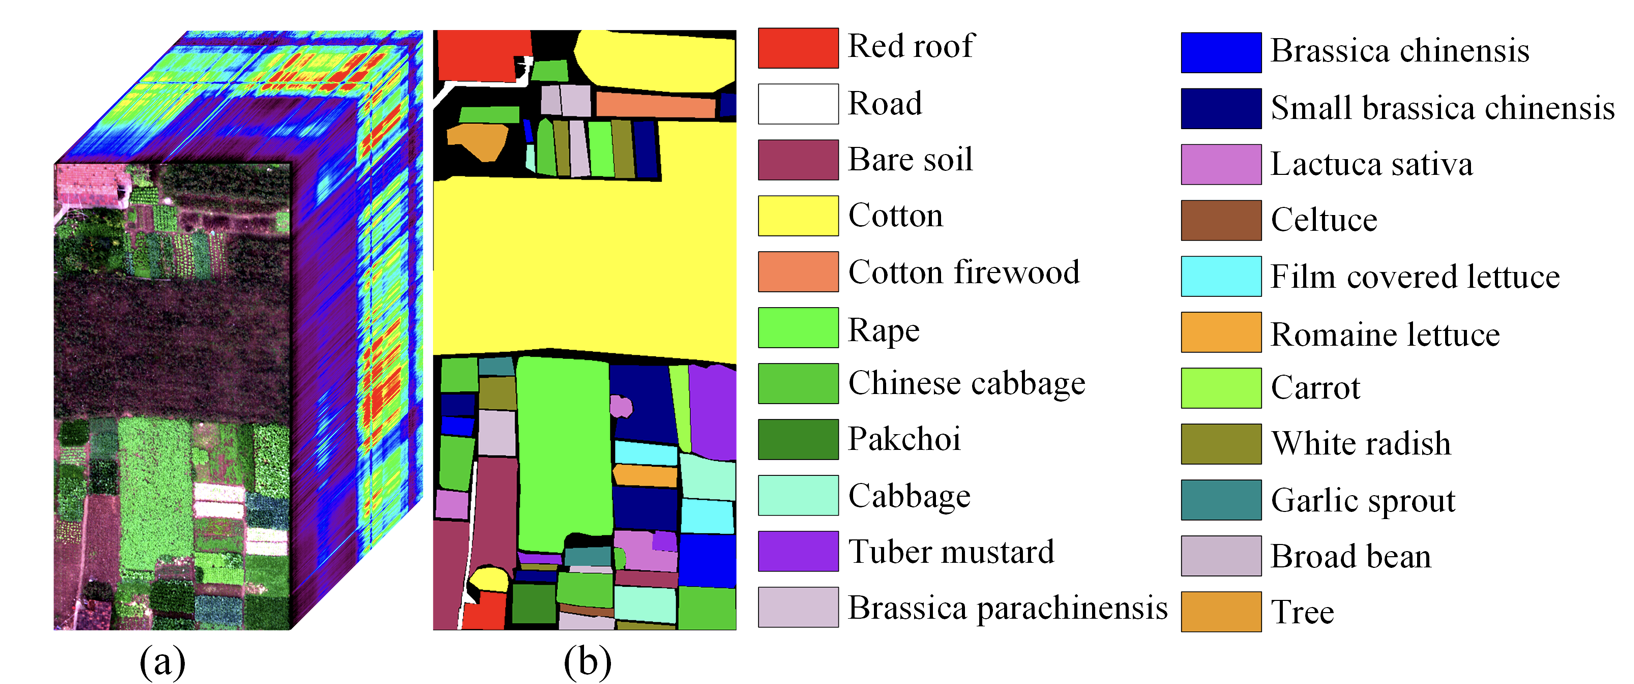
\includegraphics[width=0.62\linewidth]{WHU-Hi.png}
    \captionsetup{labelformat=simple, labelsep=colon, font=tiny, labelfont={color=gray,bf}}
    \caption{The WHU-Hi-HongHu dataset. (a) Image cube. (b) Ground-truth image.\cite{huWHUHiUAVborneHyperspectral}}
    \label{fig:WHU-Hi}
\end{figure}
\vspace{-1cm} % Adjust this value as needed to reduce the space
\begin{table}[]
    \centering
    \begin{tabular}{|p{4.5cm}|p{6cm}|p{0.5cm}|}
        \hline
        \textbf{Title (DOI)} & \textbf{Description} & \textbf{Cite} \\ \hline
        WHU-Hi: A UAV-borne Hyperspectral Image Dataset for Classification \newline \href{https://consensus.app/papers/whuhi-uavborne-resolution-benchmark-datasets-image-hu/c738ddb273815adda3d8fadfcd4f0192/?utm_source=chatgpt}{\color{blue}10.1109/TGRS.2020.2983299} & [RS] The Wuhan UAV-borne hyperspectral image dataset provides high spectral and spatial resolution data for hyperspectral image classification. & \cite{huWHUHiUAVborneHyperspectral} \\ \hline
    \end{tabular}
\end{table}
\end{frame}

\begin{frame}{Benchmark Datasets in HSI - Part 3}
\small
\begin{figure}
    \centering
    \begin{columns}[T] % Align columns at the top
        % Left column with the image
        \begin{column}{0.38\textwidth}
            \centering
            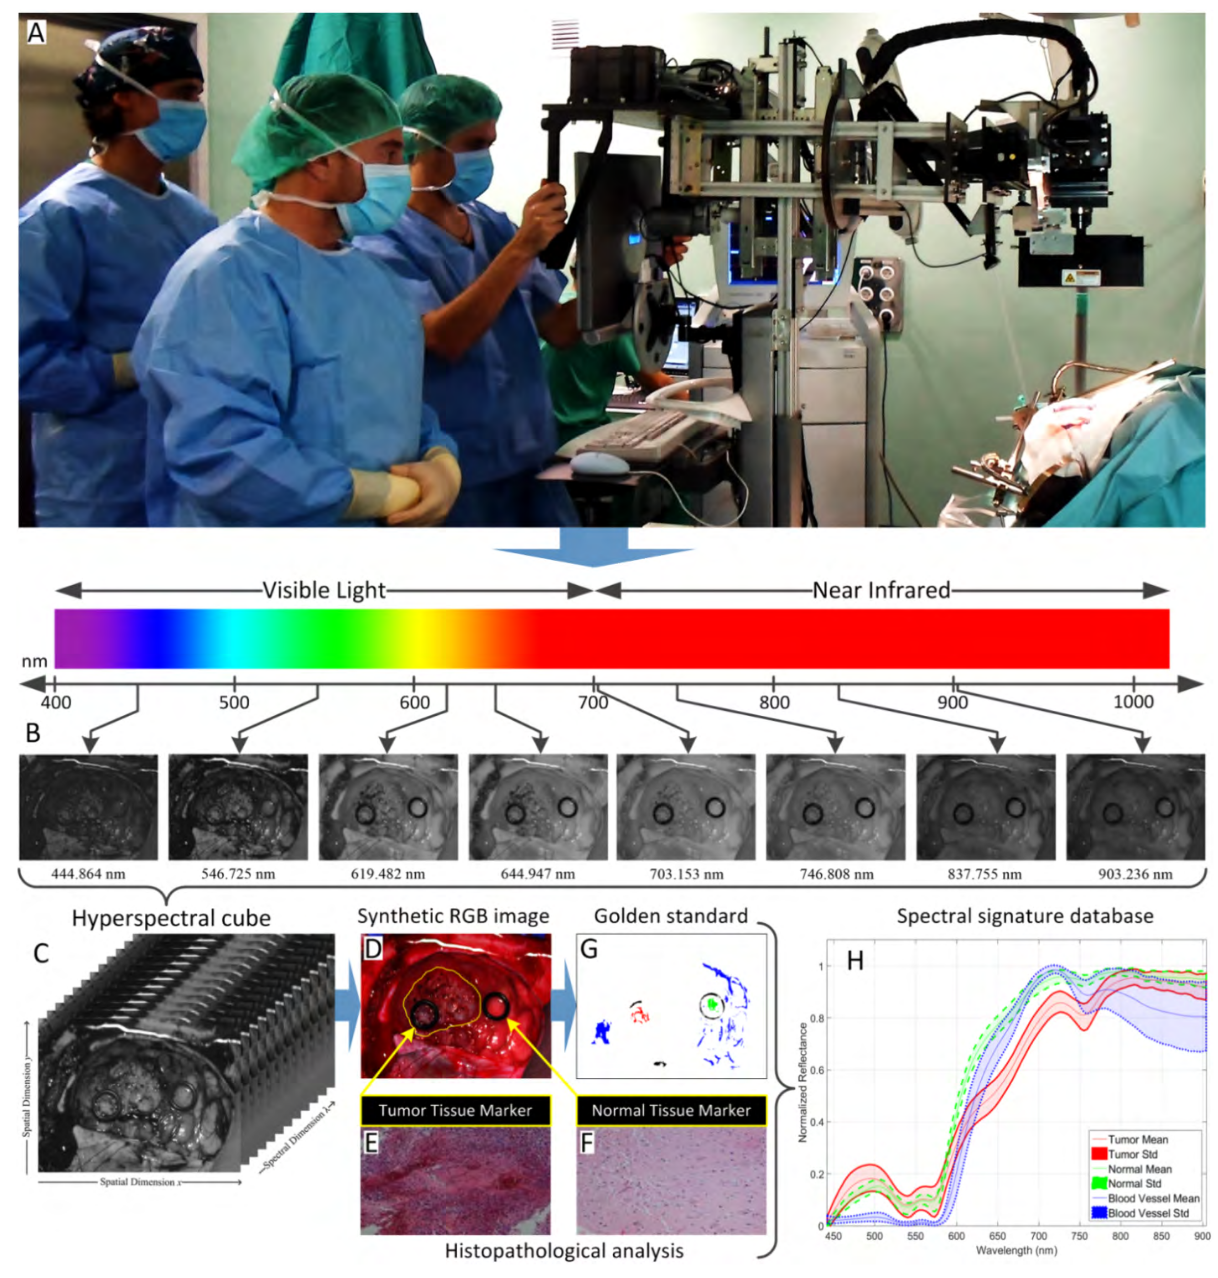
\includegraphics[width=0.8\linewidth]{In-Vivo.png}
        \end{column}
        % Right column with the caption
        \begin{column}{0.62\textwidth}
            \captionsetup{labelformat=simple, labelsep=colon, font=tiny, labelfont={color=gray,bf}}
            \caption{In-vivo HS brain surface acquisition procedure. (a) Hyperspectral acquisition system being used during the acquisition process in a neurosurgical operation. (b) Hyperspectral images acquired with the acquisition system at different wavelengths from a patient affected by a glioblastoma tumor. (c) HSI data cube. (d) RGB image generated from the HS cube with the tumor tissue marker (left) and the normal tissue marker (right) placed on the brain surface. (e) and (f) Histopathological images of the tumor tissue sample (glioblastoma) and normal tissue sample respectively. (g) Gold standard map where certain pixels have been labeled in four different classes: normal brain tissue (green), tumor tissue (red), blood vessel (blue) and background (black). (h) Average and standard deviation (Std) of the pre-processed spectral signatures of tumor tissue, normal tissue and blood vessel labeled pixels, represented in red, green and blue color respectively.\cite{fabeloInVivoHyperspectralHuman2019}}
        \end{column}
    \end{columns}
    \label{fig:In-Vivo}
\end{figure}
\vspace{-1cm} % Adjust this value as needed to reduce the space
\begin{table}[]
    \centering
    \begin{tabular}{|p{4.5cm}|p{6cm}|p{0.5cm}|}
        \hline
        \textbf{Title (DOI)} & \textbf{Description} & \textbf{Cite} \\ \hline
        In-Vivo Hyperspectral Human Brain Image Database \newline \href{https://consensus.app/papers/invivo-hyperspectral-human-brain-image-database-brain-fabelo/14753e1e2ea15718be292f660ad9ec53/?utm_source=chatgpt}{\color{blue}10.1109/TMI.2019.2926947} & [BME] Developed for brain cancer detection, this dataset includes hyperspectral images of human brain tissues acquired during neurosurgery. & \cite{fabeloInVivoHyperspectralHuman2019} \\ \hline
    \end{tabular}
\end{table}
\end{frame}

\begin{frame}{Benchmark Datasets in HSI - Part 4}
\small
\begin{table}[]
    \centering
    \begin{tabular}{|p{4.5cm}|p{6cm}|p{0.5cm}|}
        \hline
        \textbf{Title (DOI)} & \textbf{Description} & \textbf{Cite} \\ \hline
        Benchmark for Hyperspectral Unmixing Algorithm Evaluation \newline \href{https://consensus.app/papers/benchmark-hyperspectral-unmixing-algorithm-evaluation-paura/46070bf6345059e99d77d14e4dadef27/?utm_source=chatgpt}{\color{blue}10.1109/JSTARS.2023.3176657} & [RS] This dataset includes several hyperspectral images with ground truths for testing hyperspectral unmixing algorithms. & \cite{pauraBenchmarkHyperspectralUnmixing2023} \\ \hline
        Microscopic Hyperspectral Image Analysis: Datasets for Cell and Microplastics Detection \newline \href{https://consensus.app/papers/microscopic-hyperspectral-image-analysis-deep-learning-chen/aaa2e55a0cd357e6bd6615d6683789c3/?utm_source=chatgpt}{\color{blue}10.1109/TMI.2020.2975663} & [Mixed] Two benchmark datasets of cells and microplastics are used for cell classification and microplastics detection. & \cite{chenMicroscopicHyperspectralImage2020} \\ \hline
    \end{tabular}
\end{table}
\end{frame}



\section{Software Packages}
\begin{frame}{Tools for Hyperspectral Image Analysis}
\small % Reducing font size
\begin{itemize}
    \item 
\includegraphics[height=1em]{matlab_icon.png} \textbf{HYPER-Tools} (Matlab)\cite{mobarakiHYPERToolsGraphicalUserfriendly2018}: Integrates spectral and spatial preprocessing with robust analysis and visualization capabilities. Ideal for exploratory data analysis and machine learning.  \href{https://www.hypertools.org}{\color{blue}Read more}
    \item 
\includegraphics[height=1em]{matlab2_icon.png} \textbf{Hyperspectral Image Analysis Toolbox}\cite{arzuaga-cruzMATLABToolboxHyperspectral2004}: Extends Matlab for processing imagery, focusing on environmental and biomedical applications. \href{https://consensus.app/papers/matlab-toolbox-hyperspectral-image-analysis-arzuagacruz/c1ab5fe0544557e7af3de5e2ed62250a/?utm_source=chatgpt}{\color{blue}Read more}
    \item 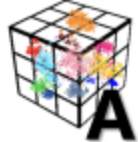
\includegraphics[height=1em]{qgis_icon.png} \textbf{AVHYAS Plugin for QGIS} \cite{lyngdohAVHYASFreeOpen2021}: Supports atmospheric correction and machine learning. Free and open-source. \href{https://sites.google.com/view/avhyas-sac-isro/home}{\color{blue}Read more}
    \item 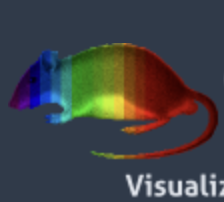
\includegraphics[height=1em]{generic_icon.png} \textbf{Gerbil} \cite{jordanNovelFrameworkInteractive2016}: An open-source framework for interactive visualization of hyperspectral data. \href{http://gerbilvis.org}{\color{blue}Read more}
    \item 
\includegraphics[height=1em]{envi_icon.png} \textbf{ENVI} \cite{xingHyperspectralImageAnalysis2001}: Commercial software for data pre-processing, analysis, and visualization. \href{hhttps://www.nv5geospatialsoftware.com/Products/ENVI}{\color{blue}Read more}
    \item 
\includegraphics[height=1em]{open_source_icon.png} \textbf{OpenSpyrit Ecosystem} \cite{benetimartinsOpenSpyritEcosystemOpen2023}: For hyperspectral single-pixel imaging, includes data acquisition and reconstruction tools. \href{https://github.com/openspyrit/spyrit}{\color{blue}Read more}
\end{itemize}
\end{frame}

\section{Kernels}
\begin{frame}{Kernels}
    \begin{table}[h]
    \centering
    \small
    \begin{tabular}{|>{\centering\arraybackslash}m{2cm}|>{\centering\arraybackslash}m{4cm}|>{\arraybackslash}m{4cm}|}
    \hline
    \textbf{Type} & \textbf{Formula} & \textbf{Properties} \\
    \hline
    Linear & $K(x, y) = x \cdot y$ & Simple linear relationship \newline Convex \\
    \hline
    Poly. & $K(x, y) = (x \cdot y + c)^d$ & \(c\) (offset), \(d\) (degree) \newline Captures polynomial features \newline Non-convex for high \(d\) \\
    \hline
    Gaussian & $K(x, y) = \exp(-\gamma \|x - y\|^2)$ & \(\gamma\) (spread) \newline Isotropic \newline Convex, smooth \\
    \hline
    Sigmoid & $K(x, y) = \tanh(\alpha x \cdot y + c)$ & \(\alpha\) (slope), \(c\) (offset) \newline Non-convex \\
    \hline
    Exp. & $K(x, y) = \exp(-|x - y|)$ & Robust to outliers \newline Convex, L1 norm-based \\
    \hline
    Laplacian & $K(x, y) = \exp\left(-\frac{|x - y|}{\sigma}\right)$ & \(\sigma\) (scale) \newline Handles varying densities \newline Convex \\
    \hline
    \end{tabular}
    \label{tab:kernels}
    \end{table}
\end{frame}


\section{Further Reading}
\begin{frame}{Further Reading}
    \frametitle{Access:}
    \begin{itemize}
        \item For more detailed information, access our GitX page:

        \begin{itemize}
            \item {\color{blue} \href{https://gitlab.oit.duke.edu/jw853/clustering4hsi}{https://gitlab.oit.duke.edu/jw853/clustering4hsi}}
            
            \item {\color{blue} \href{https://github.com/qqgjyx/CS_GroupMeeting_HSI}{https://github.com/qqgjyx/CS\_GroupMeeting\_HSI}} {\tiny (Overleaf submodel)}

            \item {\color{blue} \href{https://github.com/qqgjyx/c4h-data}{https://github.com/qqgjyx/c4h-data}} {\tiny (data worker)}

            \item {\color{blue} \href{https://github.com/qqgjyx/CS-Group}{https://github.com/qqgjyx/CS-Group}} {\tiny \color{red}(deprecated)}
        \end{itemize}
        

        \item For DEMO of early implementation:
        \begin{itemize}
            \item {\color{blue} \href{http://c4h.qqgjyx.com}{https://c4h.qqgjyx.com}}
        \end{itemize}

        
        \item Juntang's personal website:
        \begin{itemize}
            \item {\color{blue} \href{https://www.qqgjyx.com}{https://www.qqgjyx.com}}
        \end{itemize}
    \end{itemize}    
\end{frame}

\section{References}
\begin{frame}[allowframebreaks]{References}
\small
\bibliographystyle{IEEEtran}
\bibliography{HSI}
\end{frame}

\end{document}


